\documentclass[12pt]{report}
%\usepackage[a4paper, total={15cm, 20cm}]{geometry}

\usepackage{amsmath}
\usepackage{amsthm}
\usepackage{amssymb}
\usepackage{amsbsy}
\usepackage{graphicx}
\usepackage{natbib}
\usepackage{url}
\usepackage{subcaption}
\usepackage[nottoc]{tocbibind}

\DeclareMathOperator{\expfamily}{ExpFamily}
\DeclareMathOperator{\expectation}{\mathbb{E}}
\DeclareMathOperator{\variance}{\mathbb{V}ar}
\DeclareMathOperator{\cov}{\mathbb{C}ov}
\DeclareMathOperator{\corr}{\mathbb{C}orr}
\DeclareMathOperator{\bernoulli}{Bernoulli}
\DeclareMathOperator{\betaDist}{Beta}
\DeclareMathOperator{\dirichlet}{Dir}
\DeclareMathOperator{\bin}{Bin}
\DeclareMathOperator{\MN}{Multinomial}
\DeclareMathOperator{\prob}{\mathbb{P}}
\DeclareMathOperator{\trace}{Tr}
\DeclareMathOperator{\normal}{N}
\DeclareMathOperator{\gammaDist}{Gamma}
\DeclareMathOperator{\poisson}{Poisson}

\newcommand{\RSS}{\mathrm{RSS}}
\newcommand{\euler}{\mathrm{e}}
\newcommand{\diff}{\mathrm{d}}
\newcommand{\T}{^\textup{T}}
\newcommand{\dotdotdot}{_{\phantom{.}\cdots}}
\newcommand{\BIC}{\textup{BIC}}

\newcommand{\vect}[1]{\mathbf{#1}}
\newcommand{\vectGreek}[1]{\boldsymbol{#1}}
\newcommand{\matr}[1]{\mathsf{#1}}

\newtheorem{theorem}{Theorem}
\newtheorem{algorithm}{Algorithm}


\begin{document}

%=====TITLE PAGE======
\begin{titlepage}
\centering
\vspace*{1cm}
        
        \LARGE
        \textbf{Inside-Out: Characterisation of Computed Tomography Noise in Projection and Image Space with Applications to 3D Printing}
        
		\large        
        
        \vspace{2cm}
        {OxWaSP 2015-16 Warwick Cohort - Mini-project 1}
        
        \vspace{1cm}
        {Sherman Ip}

        \vspace{1cm}
        {Supervisor: Dr.~J.~Brettschneider (Statistics, Warwick)}
        
        \vspace{1cm}
        {Supervisor: Prof.~T.~Nichols (Statistics, Warwick)}
        
        \vspace{1cm}
        {10th June 2016}
\end{titlepage}

%======ABSTRACT=========
\begin{abstract}
I did this. This happened. I should of done that.
\end{abstract}

%======ACKNOWLEDGEMENT=========
\renewcommand{\abstractname}{Acknowledgements}
\begin{abstract}
None
\end{abstract}

%=====FRONT MATTER=====
\tableofcontents
%\listoffigures
%\listoftables

%======INTRODUCTION========
\chapter{Introduction}
Mini-project for OxWaSP.

%======LITERATURE REVIEW========
\chapter{Literature Review}
Computed tomography (CT) scanning is a 3D imaging technique. It does this by reconstructing the geometry of the sample through a series of 2D X-ray images of the sample. The sample rotates after each image taken.

Figure \ref{fig:x_ray_ct} shows a diagram on how CT scanning works. A 2D image is taken by projecting X-ray photons onto the stationary sample. The photons are then scattered or absobred by the sample.  Some of these photons are then detected by an X-ray detector on the other side of the sample, which produces an image. After an image has been taken, the object rotates and another image is taken. Finally after a number of images, a 3D reconstruction of the object can be estimated \cite{cantatore2011introduction}.

\begin{figure}
\centering
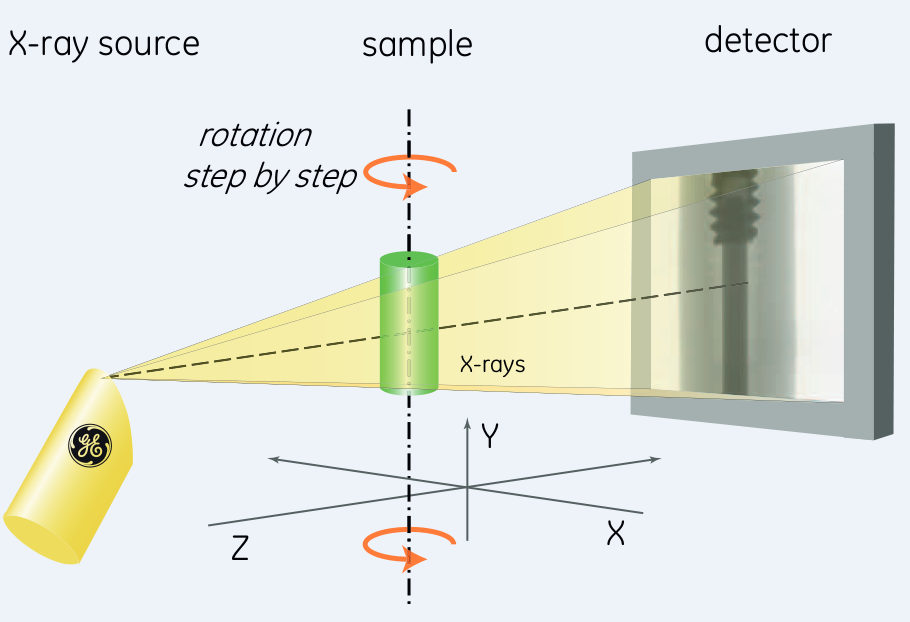
\includegraphics[width=0.7\textwidth]{figures/x_ray_ct.png}
\caption{X-ray computed tomography reconstructs the sample by projecting X-ray photons onto a rotating sample. The photon are then detected by the detector. \emph{Source: http://www.phoenix-xray.com/}}
\label{fig:x_ray_ct}
\end{figure}

CT scanning was invented by G. Hounsfield \cite{hounsfield1980computed} in the 1980's and it was mainly used for medical imaging. The setup for CT scanning is different when scanning patients because the detector and X-ray source rotates around the patient \cite{cantatore2011introduction}. Recently CT has been used industrially for non-destructive testing in manufacturing \cite{cantatore2011introduction}. One possible application would be inspecting 3D printed (additive layer manufactured) samples.

There are many sources of error in CT scanning \cite{cantatore2011introduction} and this can cause problems when reconstructing the geometry of the sample. Sources of error include: defects in the detector, environmental noise and the behaviour of photons.

This chapter aims to give brief description on how CT scanning works and a short discussion on the sources of error.

\section{X-Ray Production}
X-ray photons in CT scanning are produced in an X-ray tube. In an X-ray tube, a cathode, consisting of a heated filament, fires projectile electrons through an electric potential to a target which forms the anode \cite{michael2001x}, as shown in Figure \ref{fig:x_ray_tube}. Most of the kinetic energy of the projectile electrons is converted into heat however some is converted into electromagnetic radiation. This depends on how the projectile electrons interact with the atoms in the anode \cite{cantatore2011introduction}.

\begin{figure}
\centering
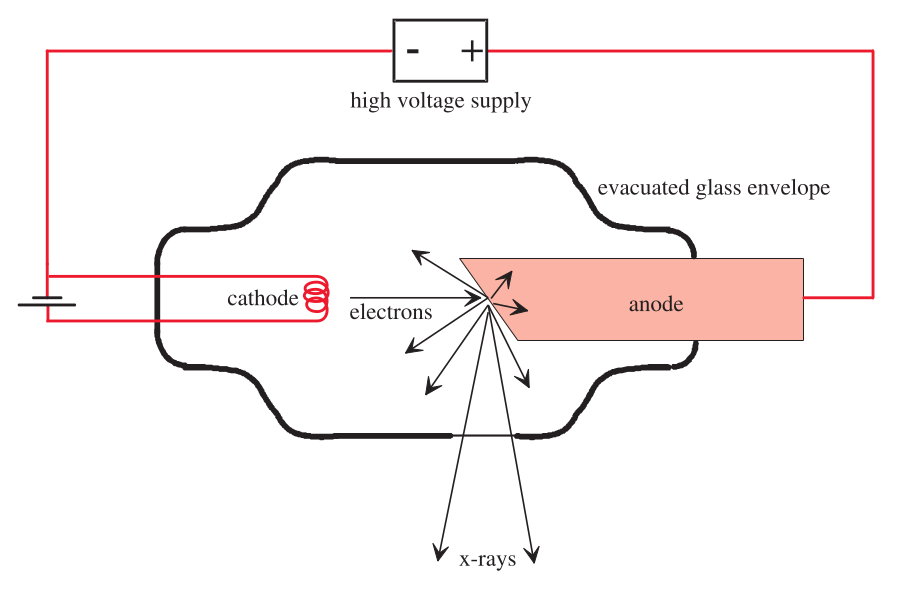
\includegraphics[width=0.8\textwidth]{figures/x_ray_tube.png}
\caption{An X-ray tube produces X-ray photons by firing projectile electrons from a cathode to an anode. \emph{Source: G.~Michael (2001) \cite{michael2001x}}}
\label{fig:x_ray_tube}
\end{figure}

Bremsstrahlung radiation is the result of projectile electrons deaccelerating due to the electrostatic field produced by nucleus of the target. The kinetic energy of the projectile electrons is then converted to electromagnetic radiation to produce X-ray radiation. As a result, the photon energies in bremsstrahlung radiation is  a continuous spectrum and can range up to the maximum kinetic energy of the projectile electrons \cite{michael2001x}.

Characteristic radiation is due to projectile electrons colliding with electrons in the target atom and ionizing them. This produce vacancies in the electron shell and emits X-ray photons when the electrons in the target atom drops down back to the ground state. The energy of the emitted radiation is monoenergetic and depends on the binding energy of the target's atoms \cite{michael2001x}.

A typical energy spectrum of X-ray photons emitted from an X-ray tube is as shown in Figure \ref{fig:x_ray_spectrum}. The energy spectrum consist of both bremsstrahlung and characteristic radiation \cite{michael2001x}.

\begin{figure}
\centering
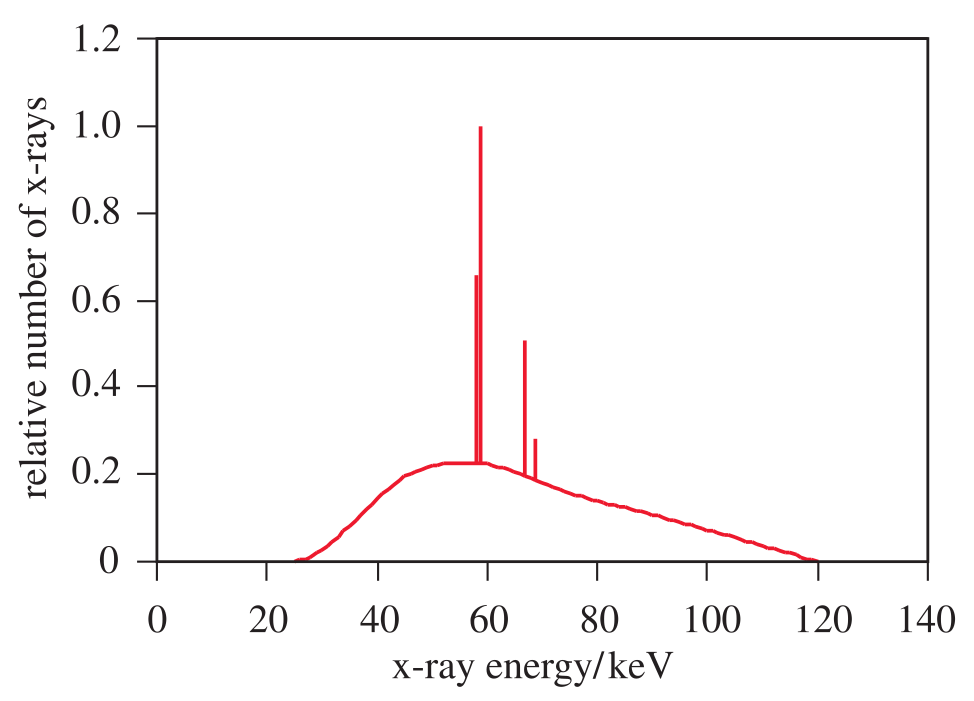
\includegraphics[width=0.8\textwidth]{figures/x_ray_spectrum.png}
\caption{A typical energy spectrum of X-ray photons emitted from an X-ray tube. The continuous spectrum is the result of Bremmsstrahlung radiation. The peaks are the result of characteristic radiation. \emph{Source: G.~Michael (2001) \cite{michael2001x}}}
\label{fig:x_ray_spectrum}
\end{figure}

The voltage, the energy per charge, and current, the rate of charge, can be varied in the X-ray tube to produce different energy spectrums and rate of X-ray emittion. This can vary the results produced when collecting CT data \cite{cantatore2011introduction}. Another important factor is the focal spot size because smaller spot sizes produce sharper edges. Larger spot sizes produce unsharp results and this is know as the penumbra effect, as shown in Figure \ref{fig:x_ray_penumbra}. However spot sizes too small can produce concentrated heat \cite{welkenhuyzen2009industrial}.

\begin{figure}
\centering
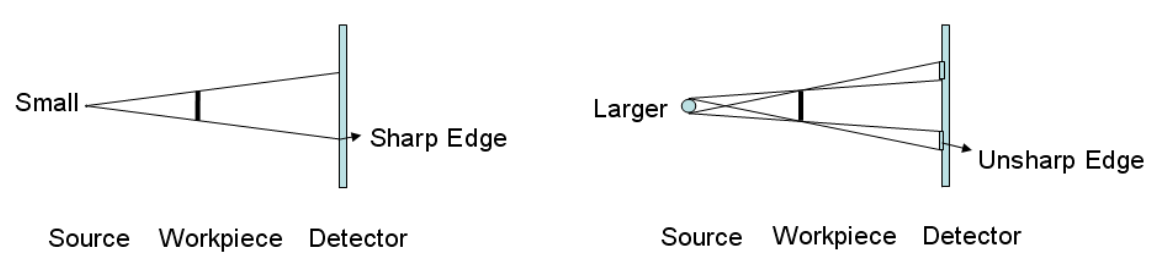
\includegraphics[width=1\textwidth]{figures/x_ray_penumbra.png}
\caption{Larger focal spot sizes produces unsharp results. This is know as the penumbra effect. \emph{Source: F.~Welkenhuyzen et al.~(2009)\cite{welkenhuyzen2009industrial}}}
\label{fig:x_ray_penumbra}
\end{figure}

\section{X-Ray Interactions}
X-ray radiation emitted by the X-ray tube are projected onto the sample and interacts with it in a number of ways \cite{cantatore2011introduction}.

The sample can effectively absorb X-ray radiation via the photoelectric effect or pair production \cite{cantatore2011introduction}. In the photoelectric effect, the X-ray photons transfers all its energy to a bounded electron and ejects it from the atom \cite{millikan1916direct}. In pair production, the X-ray photons converts into an electron-position pair by interacting with the Coulomb field of the sample's atomic nucleus \cite{hubbell2006electron}.

X-ray photons can be scattered by the sample. This happens when X-ray photons collide inelastically with and transfers it's energy to the sample's electrons. This process is know as Compton scattering \cite{compton1923quantum}.

The attenuation (decrease in X-ray intensity from $I_0$ to $I_1$) when propagating though a material with attenuation coefficient $\mu$ and distance $x$ is given as
\begin{equation}
I_1 = I_0\euler^{-\mu x}
\end{equation}
where it was assumed the X-ray photons are monoenergetic \cite{michael2001x}. This can be extended to a continuous spectrum of X-ray energies by making $\mu$ dependent on the energy of the X-ray photons \cite{cantatore2011introduction}. In general low energy photons are more likely to be absorbed than high energy photons, this increases the average energy of the attenuated photons and can be a source of error in CT scanning. This is referred to beam hardening \cite{michael2001x}. This can be reduced by placing a thin sheet of filter to absorb low energy photons \cite{welkenhuyzen2009industrial} or by correcting it in the data analysis stage \cite{michael2001x}.

\section{Detector}
Most X-ray detectors are scintillator-photodiode detectors. The X-ray photons interact with the scintiallator material and produces visible light. The visible light is then detected by photodiodes and coverts it into electricical current \cite{michael2001x}. The detectors used in CT scanning are flat bed scanner which consist of an array of panels of photodiodes \cite{cantatore2011introduction}.

\section{Reconstruction}
The scale of the 2D images are calibrated with the use of reference standards \cite{bartscher2007enhancement}. The method used to reconstruct the 3D geometry of the sample is called the filtered back-projection \cite{michael2001x}. The mathematics can be reviewed in \cite{brooks1976principles}.

\chapter{Exploratory Data Analysis}
\section{Summary Statistics}
A dataset was given for this project. It consists of 100 realizations of an X-ray image of a cuboid with its vertices in the middle, taken using an X-ray detector. These images were 1\,996$\times$1\,996 pixels in size and have a colour depth of 16 bits. A sample of them can be viewed in Figure \ref{fig:block_montage}.

\begin{figure}
\centering
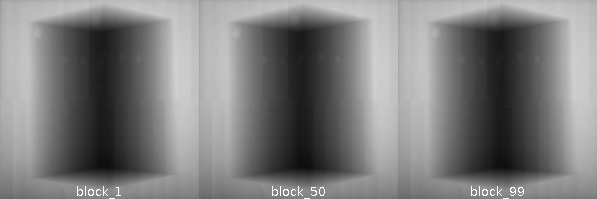
\includegraphics[width=1\textwidth]{figures/block_montage.jpg}
\caption{The 1st, 50th and 99th image in the dataset of an X-ray image of a cuboid.} 
\label{fig:block_montage}
\end{figure}

\subsection{Histogram}
The distribution of the grey values of all the pixels in the data set is shown in Figure \ref{fig:block_histogram}. It was observed that there were 3 distinct peaks in the histogram at $\sim2\times10^4$, $\sim4\times10^4$ and $\sim5\times10^4$. By doing a threshold, as shown in Figure \ref{fig:block_histogram}, it was clear that the main 3 sources of the grey values were the sample, the background and the foam holder at the bottom of the image.

\begin{figure}
\centering
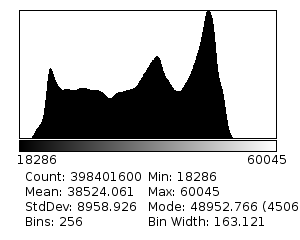
\includegraphics[width=0.5\textwidth]{figures/block_histogram.png}
\caption{Histogram of the grey values of all the pixels in the 100 images in the dataset. The grey values range from 18\,286 to 60\,045.}
\label{fig:block_histogram}
\end{figure}

\begin{figure}
	\centering
	\begin{subfigure}[b]{0.45\textwidth}
		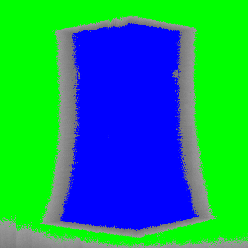
\includegraphics[width=\textwidth]{figures/block_threshold.png}
		\caption{Threshold pixels}
	\end{subfigure}
	\begin{subfigure}[b]{0.45\textwidth}
		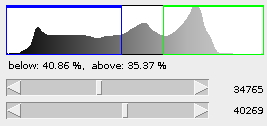
\includegraphics[]{figures/block_threshold_histogram.png}
		\caption{Histogram}	
	\end{subfigure}
	\caption{A threshold was selected to highlight pixels with different grey values. Blue: grey values less than 34\,765. Green: grey values more than 40\,269.}
	\label{fig:block_threshold}
\end{figure}

\subsection{Time Series}
The mean and standard error of the grey values for each of the 100 images were taken and plotted as a time series as shown in Figure \ref{fig:timeSeries}. There was evidence of dependence between samples by looking the sample autocorrelation plots as shown in Figure \ref{fig:timeSeries_acf_pacf}. Because there was a peak at lag 1 in the sample partial autocorrelation plot, the time series could be modelled using an autoregressive model with one parameter.

\begin{figure}
	\centering
	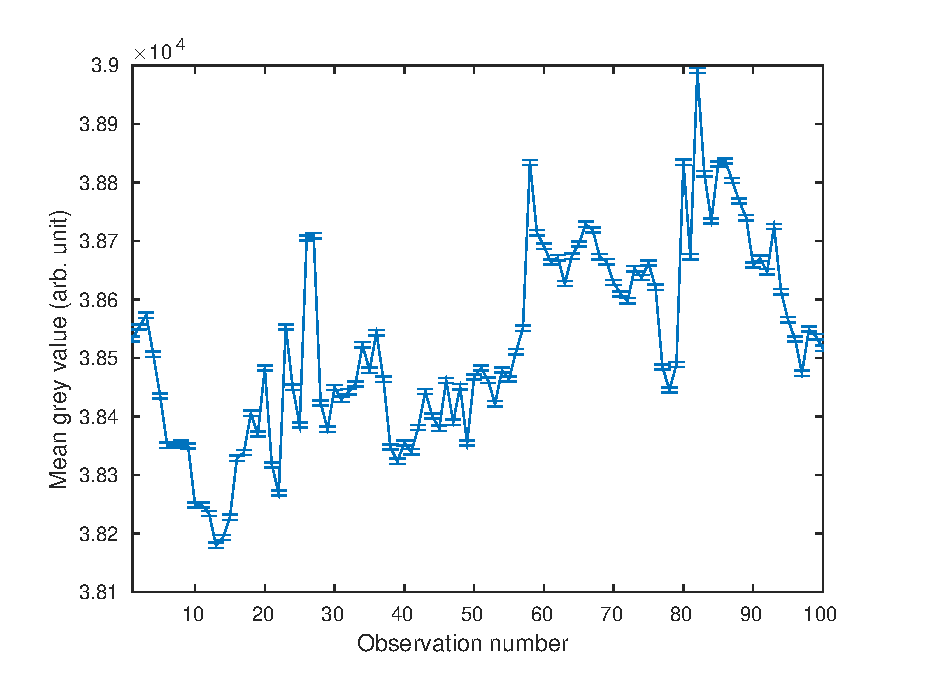
\includegraphics[width=0.75\textwidth]{figures/initial_timeSeries.eps}
	\caption{The mean and standard error of all the pixel grey values for each image.}
	\label{fig:timeSeries}
\end{figure}

\begin{figure}
	\centering
	\begin{subfigure}[b]{0.45\textwidth}
		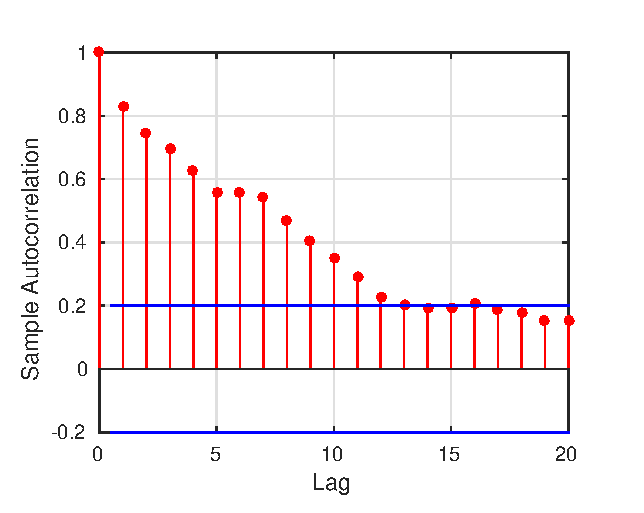
\includegraphics[width=1\textwidth]{figures/initial_acf.eps}
		\caption{Sample autocorrelation}
	\end{subfigure}
	\begin{subfigure}[b]{0.45\textwidth}
		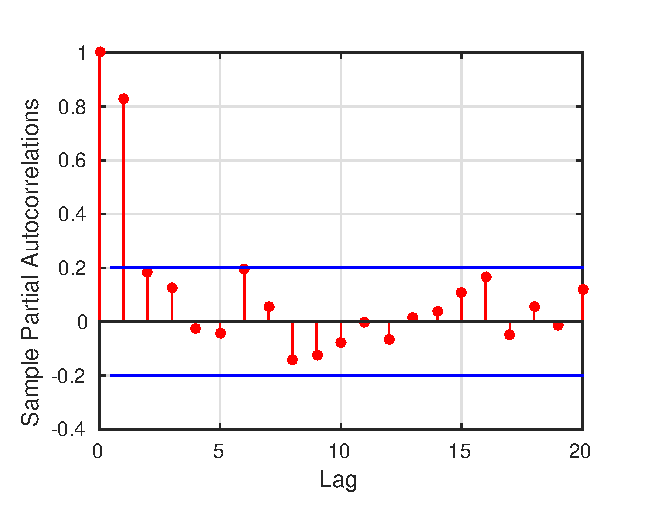
\includegraphics[width=1\textwidth]{figures/initial_pacf.eps}
		\caption{Sample partial autocorrelation}
	\end{subfigure}
	\caption{Sample autocorrelation and partial autocorrelation of the mean grey values time series.}
	\label{fig:timeSeries_acf_pacf}
\end{figure}

\subsection{Distribution of Individual Pixels}
The mean and standard deviation for each pixel's grey value was estimated and as shown in Figure \ref{fig:initial_mean_std}. Both supervised and unsupervised learning can be used to model the mean and variance relationship of the grey values.

\begin{figure}
	\centering
	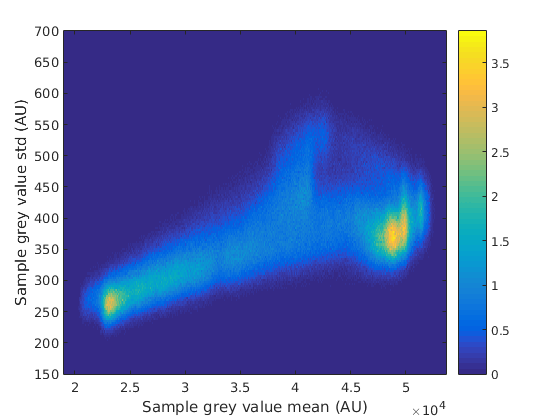
\includegraphics[width=0.9\textwidth]{figures/initial_mean_std.eps}
	\caption{Frequency density of the $1\,996^2$ pixel's grey values mean and standard deviation.}
	\label{fig:initial_mean_std}
\end{figure}

A Normal distribution was fitted on each pixel's grey values and the $\chi^2$ goodness of fit test was conducted, as shown in Figure \ref{fig:initial_fit_normal_test}. When considering the Bonferoni correction \cite{weisstein2004bonferroni} for multiple hypothesis testing, the Normal distribution appeared to be a good fit because only 9 pixels have $p$ values less than 10\%. In addition, these significant pixels did not seem to cluster and appear random in space. When ignoring the Bonferoni correction, there was a suspicious patch of low $p$ values on the bottom right.

\begin{figure}
\centering
	\begin{subfigure}[b]{0.75\textwidth}
		\includegraphics[width=1\textwidth]{figures/initial_p.eps}
		\caption{$p$ values}
	\end{subfigure}
	\begin{subfigure}[b]{0.75\textwidth}
		\includegraphics[width=1\textwidth]{figures/initial_p_log10.eps}
		\caption{$\log_{10} p$ values}
	\end{subfigure}
	\caption{$p$ values from the $\chi^2$ goodness of fit test on fitting the Normal distribution on the grey values for each pixel. In b) circled are pixels with $p$ values less than 10\%, corrected for multiple hypothesis testing using the Bonferroni correction.}
	\label{fig:initial_fit_normal_test}
\end{figure}

\section{Principal Component Analysis}
By estimating the covariance matrix of the individual pixel's grey values, sources of (orthgonal) variance can be estimated. This can be done investigating eigendecomposition representation of the sample covariance matrix. A lot of the linear algebra can be reviewed in undergraudate maths text book such as \cite{riley2006mathematical}.

\subsection{Theory}
Suppose the $p\times p$ covariance matrix $\matr{\Sigma}$ has eigenvalues $\lambda_i$ and eigenvector $\vectGreek{\phi}_i$ for $i=1,2,\dotdotdot,p$. Then the eigenvectors and eigenvalues are related by
\begin{equation}
\matr{\Sigma}\vectGreek{\phi}_i = \lambda_i\vectGreek{\phi}_i \ .
\label{eq:eigenvector_eigenvalue_forCovariance}
\end{equation}
A closure can be form by pre-multiplying both sides by $\vectGreek{\phi}_j\T$ so that
\begin{align*}
\vectGreek{\phi}_j\T \matr{\Sigma}\vectGreek{\phi}_i &= \lambda_i\vectGreek{\phi}_j\T\vectGreek{\phi}_i \\
\left(\matr{\Sigma}\T \vectGreek{\phi}_j \right)\T\vectGreek{\phi}_i &= \lambda_i\vectGreek{\phi}_j\T\vectGreek{\phi}_i \ .
\end{align*}
But given the covariance matrix is symmetric, $\matr{\Sigma}=\matr{\Sigma}\T$, and $\lambda_j$ is the corresponding eigenvalue of the eigenvector $\vectGreek{\phi}_j$, then
\begin{align*}
\left(\lambda_j\vectGreek{\phi}_j \right)\T\vectGreek{\phi}_i &= \lambda_i\vectGreek{\phi}_j\T\vectGreek{\phi}_i \\
\lambda_j\vectGreek{\phi}_j\T\vectGreek{\phi}_i &= \lambda_i\vectGreek{\phi}_j\T\vectGreek{\phi}_i \ .
\end{align*}
As long as $\lambda_i\neq\lambda_j$ for $i\neq j$, then $\vectGreek{\phi}_j\T\vectGreek{\phi}_i=0$. Therefore all eigenvalues in the covariance matrix are orthogonal to each other.

Equation \eqref{eq:eigenvector_eigenvalue_forCovariance} can be extended to include all eigenvectors and eigenvalues such that
\begin{equation}
\matr{\Sigma}
	\begin{pmatrix}
		\uparrow & \uparrow & & \uparrow \\
		\vectGreek{\phi}_1 & \vectGreek{\phi}_2 &\cdots& \vectGreek{\phi}_p \\
		\downarrow & \downarrow & & \downarrow \\
	\end{pmatrix}
=
	\begin{pmatrix}
		\uparrow & \uparrow & & \uparrow \\
		\lambda_1\vectGreek{\phi}_1 & \lambda_2\vectGreek{\phi}_2 &\cdots& \lambda_p\vectGreek{\phi}_p \\
		\downarrow & \downarrow & & \downarrow \\
	\end{pmatrix} \ .
\end{equation}
Transposing both sides
\begin{equation*}
\begin{pmatrix}
	\leftarrow\vectGreek{\phi}_1\rightarrow \\
	\leftarrow\vectGreek{\phi}_2\rightarrow \\
	\vdots \\
	\leftarrow\vectGreek{\phi}_p\rightarrow
\end{pmatrix}
\matr{\Sigma}
=
\begin{pmatrix}
	\lambda_1 & 0 & \cdots 0 \\
	0 & \lambda_2 & \cdots 0 \\
	\vdots & \vdots & \ddots \\
	0 & 0 & \cdots \lambda_p \\
\end{pmatrix}
\begin{pmatrix}
	\leftarrow\vectGreek{\phi}_1\rightarrow \\
	\leftarrow\vectGreek{\phi}_2\rightarrow \\
	\vdots \\
	\leftarrow\vectGreek{\phi}_p\rightarrow
\end{pmatrix}
\end{equation*}
but because all eigenvectors are orthogonal
\begin{equation*}
\matr{\Sigma}
=
\begin{pmatrix}
		\uparrow & \uparrow & & \uparrow \\
		\vectGreek{\phi}_1 & \vectGreek{\phi}_2 &\cdots& \vectGreek{\phi}_p \\
		\downarrow & \downarrow & & \downarrow \\
\end{pmatrix}
\begin{pmatrix}
	\lambda_1 & 0 & \cdots 0 \\
	0 & \lambda_2 & \cdots 0 \\
	\vdots & \vdots & \ddots \\
	0 & 0 & \cdots \lambda_p \\
\end{pmatrix}
\begin{pmatrix}
	\leftarrow\vectGreek{\phi}_1\rightarrow \\
	\leftarrow\vectGreek{\phi}_2\rightarrow \\
	\vdots \\
	\leftarrow\vectGreek{\phi}_p\rightarrow
\end{pmatrix} \ .
\end{equation*}
This is just a weighted sum of the outer products of the eigenvectors, therefore the eigendecomposition is
\begin{equation}
\matr{\Sigma} = \sum_{i=1}^{p} \lambda_i \vectGreek{\phi}_i \vectGreek{\phi}_i\T \ .
\end{equation}
Because this is a weighted sum, the eigenvectors with the biggest eigenvalue will be most responsible for the covariance matrix. $\vectGreek{\phi}_i$ are called the principle components.

\subsection{Methods}
The 100 images were shrunk with averaging to a size of $100\times100$ pixels using ImageJ. The sample covariance matrix, of the pixel's grey values, was calculated using the maximum likelihood estimator so that the 6 eigenvectors with the biggest eigenvalues can be obtained. Using 1\,600 bootstrap samples, the sampling distribution of the 6 eigenvalues were sampled.

\subsection{Results}
Figure \ref{fig:initial_PC_eigenvalues} shows the first 6 of the diagonal of the outer product of the individual principle components, they represent the normalised main sources of variance. It was observed that on the first and second principle components, there are sources of variance in the bottom right and top right of the image. This could imply that the sources of variance are not uniformly distributed in the background.

The sampling distribution of the eigenvalues are shown in Figure \ref{fig:initial_PC_eigenvalues}. Quite clearly there were 2 significant sources of variance because the eigenvalues of the first 2 principle components were much larger than zero when comparing it with its interquartile range.

\begin{figure}
	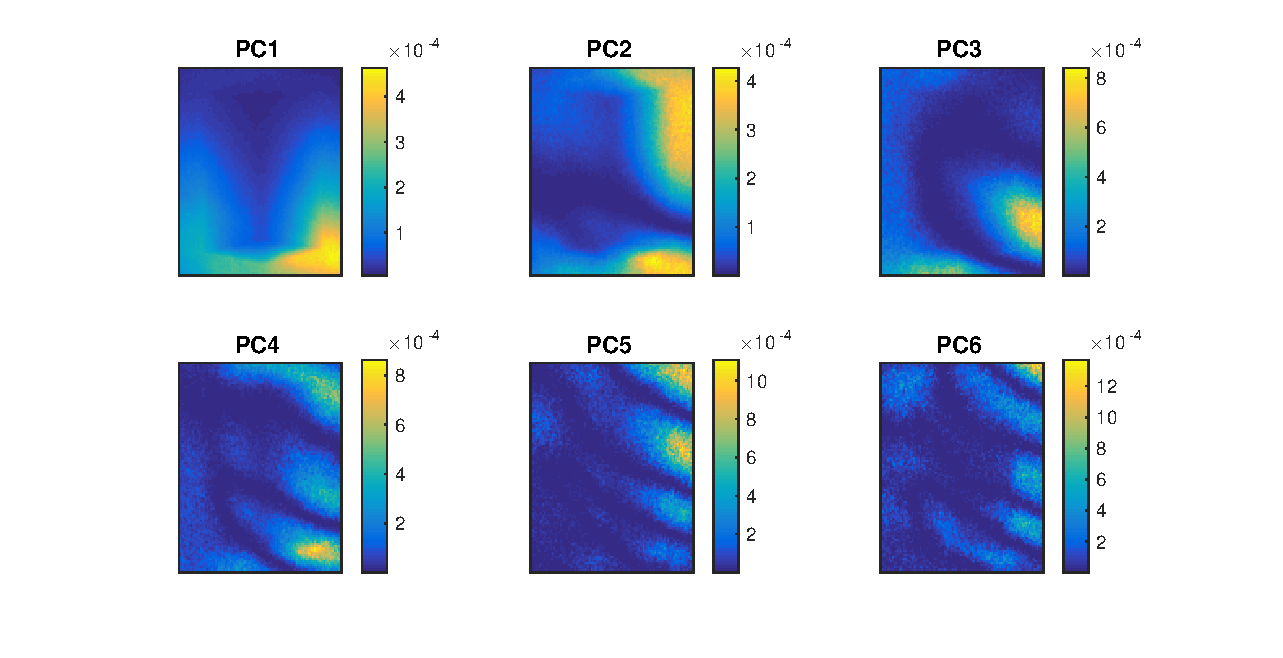
\includegraphics[width=\textwidth]{figures/initial_PCvariance.eps}
	\caption{Normalised variance due to the principle components (1 to 6). The values of all the pixels in the figures equal to 1.}
	\label{fig:initial_PCvariance}
\end{figure}
\begin{figure}
	\centering
	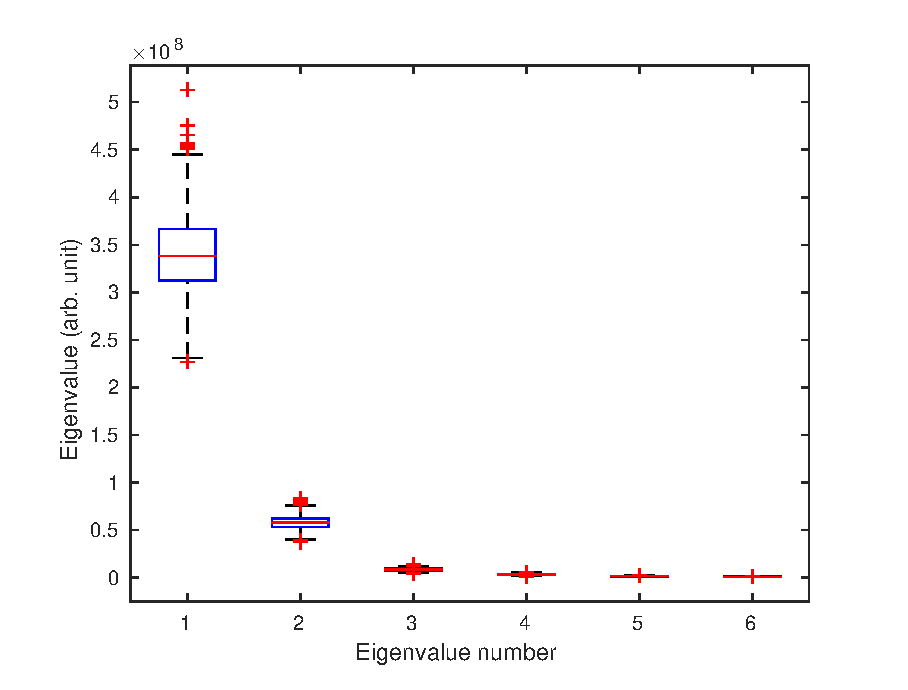
\includegraphics[width=0.7\textwidth]{figures/initial_PC_eigenvalues.eps}
	\caption{Eigenvalues of the sample covariance matrix. 1\,600 bootstrap samples were used.}
	\label{fig:initial_PC_eigenvalues}
\end{figure}

\section{Factor Analysis}
A probabilistic latent model can be used to model the pixel's grey values. These latent variables then can be used to describe the underlining structure, and perhaps sources of variance.

\subsection{Theory}
Let $\vect{Y}$ be a random vector containing $k$ latent variables, called factors, and
\begin{equation}
\vect{Y}\sim\normal\left(\vect{0},\matr{1}\right) \ .
\end{equation}
Let $\vect{e}$ be a random $p$ vector modelling the uncorrelated intrinsic noise such that
\begin{equation}
\vect{e}\sim\normal\left(\vect{0},\matr{\Psi}\right)
\end{equation}
where $\matr{\Psi}$ is a diagonal matrix.

Given a $p\times k$ loading matrix $\matr{\Lambda}$, the observable data $\vect{X}$ can be modelled through
\begin{equation}
\vect{X}=\matr{\Lambda}\vect{Y}+\vect{e}
\end{equation}
thus
\begin{equation}
\vect{X}\sim\normal\left(\vect{0},\matr{\Lambda}\matr{\Lambda}\T+\matr{\Psi}\right) \ .
\end{equation}
As a result there are two sources of variance, factor noise from the $\matr{\Lambda}\matr{\Lambda}\T$ component and the instrinic noise $\matr{\Psi}$. The model can be extended for non-zero mean easily by adding an arbitrary constant.

The conditional distribution of $\vect{X}$ given $\vect{Y}$ can be calculated to be
\begin{equation}
\vect{X}|\vect{Y}\sim\normal\left(\matr{\Lambda}\vect{Y},\matr{\Psi}\right) \ .
\label{eq:factor_analysis_x_given_y_dist}
\end{equation}
Using Bayes' theorem, the conditional distribution of $\vect{Y}$ given $\vect{X}$ can be calculated
\begin{align*}
p_{\vect{Y}|\vect{X}}(\vect{y}|\vect{x}) &\propto p_{\vect{X}|\vect{Y}}(\vect{x}|\vect{y}) p_{\vect{Y}}(\vect{y})
\\
p_{\vect{Y}|\vect{X}}(\vect{y}|\vect{x}) &\propto \exp\left[-\frac{1}{2}\left(\vect{x}-\matr{\Lambda}\vect{y}\right)\T\matr{\Psi}^{-1}\left(\vect{x}-\matr{\Lambda}\vect{y}\right)\right]
\exp\left[-\frac{1}{2}\vect{y}\T\vect{y}\right]
\\
p_{\vect{Y}|\vect{X}}(\vect{y}|\vect{x}) &\propto \exp \left[-\frac{1}{2}\left(-\vect{x}\T\matr{\Psi}^{-1}\matr{\Lambda}\vect{y}-\vect{y}\T\matr{\Lambda}\T\matr{\Psi}^{-1}\vect{x}+\vect{y}\T\matr{\Lambda}\T\matr{\Psi}^{-1}\matr{\Lambda}\vect{y}+\vect{y}\T\vect{y}\right)\right]
\\
p_{\vect{Y}|\vect{X}}(\vect{y}|\vect{x}) &\propto \exp \left[-\frac{1}{2}\left(\vect{y}\T\left(\matr{\Lambda}\T\matr{\Psi}^{-1}\matr{\Lambda}+\matr{1}\right)\vect{y}-2\vect{y}\T\matr{\Lambda}\T\matr{\Psi}^{-1}\vect{x}\right)\right]
\end{align*}
and comparing it with the density function of a general multivariate Normal distribution
\begin{equation}
\vect{Y}|\vect{X}\sim\normal\left(\left(\matr{\Lambda}\T\matr{\Psi}^{-1}\matr{\Lambda}+\matr{1}\right)^{-1}\matr{\Lambda}\T\matr{\Psi}^{-1}\vect{X},\left(\matr{\Lambda}\T\matr{\Psi}^{-1}\matr{\Lambda}+\matr{1}\right)^{-1}\right) \ .
\label{eq:factor_analysis_y_given_x_dist}
\end{equation}

Suppose $\vect{X}=\vect{x}^{(i)}$ was observed for $i=1,2,\dotdotdot,n$, then the likelihood is
\begin{equation}
L=\prod_{i=1}^n\frac{1}{{\|2\pi\left(\matr{\Lambda}\matr{\Lambda}\T+\matr{\Psi}\right)\|}^{1/2}}
\exp\left[-\frac{1}{2}\left(\vect{x}^{(i)}\right)\T\left(\matr{\Lambda}\matr{\Lambda}\T+\matr{\Psi}\right)^{-1}\vect{x}^{(i)}\right] \ .
\end{equation}
The log likelihood is then
\begin{equation*}
\ln{L}=-\frac{n}{2}\ln{\|2\pi\left(\matr{\Lambda}\matr{\Lambda}\T+\matr{\Psi}\right)\|}-\frac{1}{2}\sum_{i=1}^{n}\left(\vect{x}^{(i)}\right)\T\left(\matr{\Lambda}\matr{\Lambda}\T+\matr{\Psi}\right)^{-1}\vect{x}^{(i)}
\end{equation*}
and by using the trace and its properties
\begin{align}
\ln{L}&=-\frac{n}{2}\ln{\|2\pi\left(\matr{\Lambda}\matr{\Lambda}\T+\matr{\Psi}\right)\|}-\frac{1}{2}\sum_{i=1}^{n}\trace\left[\left(\vect{x}^{(i)}\right)\T\left(\matr{\Lambda}\matr{\Lambda}\T+\matr{\Psi}\right)^{-1}\vect{x}^{(i)}\right]
\nonumber \\
\ln{L}&=-\frac{n}{2}\ln{\|2\pi\left(\matr{\Lambda}\matr{\Lambda}\T+\matr{\Psi}\right)\|}-\frac{1}{2}\sum_{i=1}^{n}\trace\left[\left(\matr{\Lambda}\matr{\Lambda}\T+\matr{\Psi}\right)^{-1}\vect{x}^{(i)}\left(\vect{x}^{(i)}\right)\T\right]
\nonumber \\
\ln{L}&=-\frac{n}{2}\ln{\|2\pi\left(\matr{\Lambda}\matr{\Lambda}\T+\matr{\Psi}\right)\|}-\frac{1}{2}\trace\left[\left(\matr{\Lambda}\matr{\Lambda}\T+\matr{\Psi}\right)^{-1}\sum_{i=1}^{n}\vect{x}^{(i)}\left(\vect{x}^{(i)}\right)\T\right] \ .
\end{align}
The loading matrix $\matr{\Lambda}$ and intrinsic noise $\matr{\Psi}$ can be estimated by maximising the log likelihood. This is best done using the expectation maximisation (EM) algorithm. The EM algorithm is an iterative procedure conducting an E step followed by a M step many times till some convergence conditions are met.

The E step estimates the values of the latent variables, $\vect{y}^{(1)},\vect{y}^{(2)},\dotdotdot,\vect{y}^{(n)}$, using the expectation of the condition distribution of the latent variables given the observed data $\vect{x}^{(1)},\vect{x}^{(2)},\dotdotdot,\vect{x}^{(n)}$. The parameters $\matr{\Lambda}$ and $\matr{\Psi}$ are assumed to be know in this step and are fixed. By using Equation \eqref{eq:factor_analysis_y_given_x_dist}, each latent variable are assigned by
\begin{equation}
\vect{y}^{(i)} \leftarrow \left(\matr{\Lambda}\T\matr{\Psi}^{-1}\matr{\Lambda}+\matr{1}\right)^{-1}\matr{\Lambda}\T\matr{\Psi}^{-1}\vect{x}^{(i)}
\end{equation}
for $i=1,2,\dotdotdot,n$. The covariance of the latent variables are estimated by
\begin{equation}
\matr{\Sigma}_{\vect{Y}} \leftarrow \left(\matr{\Lambda}\T\matr{\Psi}^{-1}\matr{\Lambda}+\matr{1}\right)^{-1}
\end{equation}

In the E step, the parameters $\matr{\Lambda}$ and $\matr{\Psi}$ are varied to maximise the log likelihood, assuming the latent variables are known and fixed. The objective to maximise is the condition expectation of the log joint likelihood, this is given as
\begin{equation}
H = \expectation_{\vect{Y}|\vect{X}}\left[\sum_{i=1}^{n}\ln p_{\vect{X},\vect{Y}}\left(\vect{x}^{(i)},\vect{y}^{(i)}\right)\right] \ .
\end{equation}
This can be expressed as
\begin{equation*}
H = \expectation_{\vect{Y}|\vect{X}}\left[
\sum_{i=1}^{n}\left(\ln p_{\vect{X}|\vect{Y}}\left(\vect{x}^{(i)}|\vect{y}^{(i)}\right)+\ln p_{\vect{Y}}\left(\vect{y}^{(i)}\right)\right)
\right]
\end{equation*}
Because the marginal distribution of the latent variables do not depend on $\matr{\Lambda}$ and $\matr{\Psi}$, this can be ignored. Using Equation \eqref{eq:factor_analysis_x_given_y_dist}
\begin{equation*}
H = \expectation_{\vect{Y}|\vect{X}}\left[
\sum_{i=1}^{n}\ln\left(\frac{1}{\|2\pi\matr{\Psi}\|^{1/2}}\exp\left(-\frac{1}{2}\left(\vect{x}^{(i)}-\matr{\Lambda}\vect{y}^{(i)}\right)\T\matr{\Psi}^{-1}\left(\vect{x}^{(i)}-\matr{\Lambda}\vect{y}^{(i)}\right)\right)\right)
\right]
+c_1
\end{equation*}
\begin{equation*}
H = \expectation_{\vect{Y}|\vect{X}}\left[
\sum_{i=1}^{n}\left(-\frac{1}{2}\ln{\|2\pi\matr{\Psi}\|}-\frac{1}{2}\left(\vect{x}^{(i)}-\matr{\Lambda}\vect{y}^{(i)}\right)\T\matr{\Psi}^{-1}\left(\vect{x}^{(i)}-\matr{\Lambda}\vect{y}^{(i)}\right)\right)
\right]
+c_1
\end{equation*}
\begin{equation*}
H = -\frac{1}{2}\expectation_{\vect{Y}|\vect{X}}\left[
\sum_{i=1}^{n}\left(\ln{\|2\pi\matr{\Psi}\|}+\left(\vect{x}^{(i)}\right)\T\matr{\Psi}^{-1}\matr{\Lambda}\vect{y}^{(i)}-2\left(\vect{x}^{(i)}\right)\T\matr{\Psi}^{-1}\matr{\Lambda}\vect{y}^{(i)}+\left(\vect{y}^{(i)}\right)\T\matr{\Lambda}\T\matr{\Psi}^{-1}\matr{\Lambda}\vect{y}^{(i)}\right)
\right]
+c_1
\end{equation*}
By defining
\begin{equation}
\expectation_{\vect{Y}|\vect{X}}\left[\vect{y}^{(i)}\right]=\vectGreek{\mu}^{(i)} = \left(\matr{\Lambda}\T\matr{\Psi}^{-1}\matr{\Lambda}+\matr{1}\right)^{-1}\matr{\Lambda}\T\matr{\Psi}^{-1}\vect{x}^{(i)}
\end{equation}
and
\begin{equation}
\cov{\vect{Y}} = \matr{\Sigma}_{\vect{Y}} = \left(\matr{\Lambda}\T\matr{\Psi}^{-1}\matr{\Lambda}+\matr{1}\right)^{-1}
\end{equation}
then when taking the conditional expectation
\begin{multline*}
H = -\frac{1}{2}\sum_{i=1}^{n}\left[
\ln\|2\pi\matr{\Psi}\|+\left(\vect{x}^{(i)}\right)\T\matr{\Psi}^{-1}\vect{x}^{(i)}-2\left(\vect{x}^{(i)}\right)\T\matr{\Psi}^{-1}\matr{\Lambda}\vectGreek{\mu}^{(i)}\right.\\
\left.+\trace\left(\matr{\Lambda}\T\matr{\Psi}^{-1}\matr{\Lambda}\matr{\Sigma}_{\vect{Y}}\right)+\left(\vectGreek{\mu}^{(i)}\right)\T\matr{\Lambda}\T\matr{\Psi}^{-1}\matr{\Lambda}\vectGreek{\mu}^{(i)}
\right]+c_1
\end{multline*}
\begin{multline*}
H = -\frac{1}{2}\sum_{i=1}^{n}\left[
\ln\|2\pi\matr{\Psi}\|+\left(\vect{x}^{(i)}\right)\T\matr{\Psi}^{-1}\vect{x}^{(i)}-2\left(\vect{x}^{(i)}\right)\T\matr{\Psi}^{-1}\matr{\Lambda}\vectGreek{\mu}^{(i)}\right.\\
\left.+\trace\left(\matr{\Lambda}\T\matr{\Psi}^{-1}\matr{\Lambda}\matr{\Sigma}_{\vect{Y}}\right)+\trace\left(\matr{\Lambda}\T\matr{\Psi}^{-1}\matr{\Lambda}\vectGreek{\mu}^{(i)}\left(\vectGreek{\mu}^{(i)}\right)\T\right)
\right]+c_1
\end{multline*}
\begin{multline*}
H = -\frac{1}{2}\sum_{i=1}^{n}\left[
\ln\|2\pi\matr{\Psi}\|+\left(\vect{x}^{(i)}\right)\T\matr{\Psi}^{-1}\vect{x}^{(i)}-2\left(\vect{x}^{(i)}\right)\T\matr{\Psi}^{-1}\matr{\Lambda}\vectGreek{\mu}^{(i)}\right.\\
\left.+\trace\left(\matr{\Lambda}\T\matr{\Psi}^{-1}\matr{\Lambda}\left(\matr{\Sigma}_{\vect{Y}}+\vectGreek{\mu}^{(i)}\left(\vectGreek{\mu}^{(i)}\right)\T\right)\right)
\right]+c_1
\end{multline*}
\begin{multline*}
H = -\frac{n}{2}
\ln\|\matr{\Psi}\|
-\frac{1}{2}\sum_{i=1}^{n}\left(\vect{x}^{(i)}\right)\T\matr{\Psi}^{-1}\vect{x}^{(i)}
+\sum_{i=1}^{n}\left(\vect{x}^{(i)}\right)\T\matr{\Psi}^{-1}\matr{\Lambda}\vectGreek{\mu}^{(i)}\\
-\frac{1}{2}\sum_{i=1}^{n}\trace\left(\matr{\Lambda}\T\matr{\Psi}^{-1}\matr{\Lambda}\left(\matr{\Sigma}_{\vect{Y}}+\vectGreek{\mu}^{(i)}\left(\vectGreek{\mu}^{(i)}\right)\T\right)\right)
+c_2
\end{multline*}

Taking the derivative with respect to $\matr{\Lambda}$
\begin{equation*}
\matr{D}_{\matr{\Lambda}}H=
\matr{D}_{\matr{\Lambda}}\left[
\sum_{i=1}^n\left(\vect{x}^{(i)}\right)\T\matr{\Psi}^{-1}\matr{\Lambda}\vectGreek{\mu}^{(i)}
-\frac{1}{2}\sum_{i=1}^{n}\trace\left(\matr{\Lambda}\T\matr{\Psi}^{-1}\matr{\Lambda}\left(\matr{\Sigma}_{\vect{Y}}+\vectGreek{\mu}^{(i)}\left(\vectGreek{\mu}^{(i)}\right)\T\right)\right)
\right]
\end{equation*}
\begin{equation*}
\matr{D}_{\matr{\Lambda}}H=
\matr{D}_{\matr{\Lambda}}\left[
\sum_{i=1}^n\trace\left(\left(\vectGreek{\mu}^{(i)}\right)\T\matr{\Lambda}\T\matr{\Psi}^{-1}\vect{x}^{(i)}\right)
-\frac{1}{2}\sum_{i=1}^{n}\trace\left(\matr{\Lambda}\T\matr{\Psi}^{-1}\matr{\Lambda}\left(\matr{\Sigma}_{\vect{Y}}+\vectGreek{\mu}^{(i)}\left(\vectGreek{\mu}^{(i)}\right)\T\right)\right)
\right]
\end{equation*}
\begin{equation*}
\matr{D}_{\matr{\Lambda}}H=
\matr{D}_{\matr{\Lambda}}\left[
\sum_{i=1}^n\trace\left(\matr{\Lambda}\T\matr{\Psi}^{-1}\vect{x}^{(i)}\left(\vectGreek{\mu}^{(i)}\right)\T\right)
-\frac{1}{2}\sum_{i=1}^{n}\trace\left(\matr{\Lambda}\T\matr{\Psi}^{-1}\matr{\Lambda}\left(\matr{\Sigma}_{\vect{Y}}+\vectGreek{\mu}^{(i)}\left(\vectGreek{\mu}^{(i)}\right)\T\right)\right)
\right]
\end{equation*}
\begin{equation*}
\matr{D}_{\matr{\Lambda}}H=
\sum_{i=1}^n\matr{\Psi}^{-1}\vect{x}^{(i)}\left(\vectGreek{\mu}^{(i)}\right)\T
-\sum_{i=1}^{n}\matr{\Psi}^{-1}\matr{\Lambda}\left(\matr{\Sigma}_{\vect{Y}}+\vectGreek{\mu}^{(i)}\left(\vectGreek{\mu}^{(i)}\right)\T\right) \ .
\end{equation*}
Setting the derivative to zero
\begin{equation*}
\matr{0}=
\sum_{i=1}^n\matr{\Psi}^{-1}\vect{x}^{(i)}\left(\vectGreek{\mu}^{(i)}\right)\T
-\sum_{i=1}^{n}\matr{\Psi}^{-1}\matr{\Lambda}\left(\matr{\Sigma}_{\vect{Y}}+\vectGreek{\mu}^{(i)}\left(\vectGreek{\mu}^{(i)}\right)\T\right) \ .
\end{equation*}
\begin{equation*}
\matr{0}=
\sum_{i=1}^n\vect{x}^{(i)}\left(\vectGreek{\mu}^{(i)}\right)\T
-\matr{\Lambda}\left(n\matr{\Sigma}_{\vect{Y}}+\sum_{i=1}^{n}\vectGreek{\mu}^{(i)}\left(\vectGreek{\mu}^{(i)}\right)\T\right)
\end{equation*}
\begin{equation}
\matr{\Lambda}
=
\left(\sum_{i=1}^n\vect{x}^{(i)}\left(\vectGreek{\mu}^{(i)}\right)\T\right)\left(n\matr{\Sigma}_{\vect{Y}}+\sum_{i=1}^{n}\vectGreek{\mu}^{(i)}\left(\vectGreek{\mu}^{(i)}\right)\T\right)^{-1}\ .
\end{equation}

The objective can be re-parametrised using $\matr{T}=\matr{\Psi}^{-1}$ so that
\begin{multline*}
H = -\frac{n}{2}
\ln\|\matr{T^{-1}}\|
-\frac{1}{2}\sum_{i=1}^{n}\left(\vect{x}^{(i)}\right)\T\matr{T}\vect{x}^{(i)}
+\sum_{i=1}^{n}\left(\vect{x}^{(i)}\right)\T\matr{T}\matr{\Lambda}\vectGreek{\mu}^{(i)}\\
-\frac{1}{2}\sum_{i=1}^{n}\trace\left(\matr{\Lambda}\T\matr{T}\matr{\Lambda}\left(\matr{\Sigma}_{\vect{Y}}+\vectGreek{\mu}^{(i)}\left(\vectGreek{\mu}^{(i)}\right)\T\right)\right)
+c_2
\end{multline*}
\begin{multline*}
H = -\frac{n}{2}
\ln\|\matr{T^{-1}}\|
-\frac{1}{2}\sum_{i=1}^{n}\left(\vect{x}^{(i)}\right)\T\matr{T}\vect{x}^{(i)}
+\sum_{i=1}^{n}\left(\vect{x}^{(i)}\right)\T\matr{T}\matr{\Lambda}\vectGreek{\mu}^{(i)}\\
-\frac{1}{2}\sum_{i=1}^{n}\trace\left(\matr{\Lambda}\T\matr{T}\matr{\Lambda}\left(\matr{\Sigma}_{\vect{Y}}+\vectGreek{\mu}^{(i)}\left(\vectGreek{\mu}^{(i)}\right)\T\right)\right)
+c_2 \ .
\end{multline*}
$\|\matr{T}^{-1}\| = 1/\|\matr{T}\|$ and using the properties of the trace
\begin{multline*}
H = \frac{n}{2}
\ln\|\matr{T}\|
-\frac{1}{2}\sum_{i=1}^{n}\trace\left(\matr{T}\vect{x}^{(i)}\left(\vect{x}^{(i)}\right)\T\right)
+\sum_{i=1}^{n}\trace\left(\matr{T}\matr{\Lambda}\vectGreek{\mu}^{(i)}\left(\vect{x}^{(i)}\right)\T\right)\\
-\sum_{i=1}^{n}\frac{1}{2}\trace\left(\matr{T}\matr{\Lambda}\left(\matr{\Sigma}_{\vect{Y}}+\vectGreek{\mu}^{(i)}\left(\vectGreek{\mu}^{(i)}\right)\T\right)\matr{\Lambda}\T\right)
+c_2 \ .
\end{multline*}
Taking the derivative with respect to $\matr{\Psi}$
\begin{multline*}
\matr{D}_{\matr{\Psi}}H = \frac{n}{2}\matr{T}^{-1}
-\frac{1}{2}\sum_{i=1}^{n}\vect{x}^{(i)}\left(\vect{x}^{(i)}\right)\T
+\sum_{i=1}^{n}\matr{\Lambda}\vectGreek{\mu}^{(i)}\left(\vect{x}^{(i)}\right)\T\\
-\sum_{i=1}^{n}\frac{1}{2}\matr{\Lambda}\left(\matr{\Sigma}_{\vect{Y}}+\vectGreek{\mu}^{(i)}\left(\vectGreek{\mu}^{(i)}\right)\T\right)\matr{\Lambda}\T \ .
\end{multline*}
Setting the derivative to zero
\begin{multline*}
\matr{0} = \frac{n}{2}\matr{\Psi}
-\frac{1}{2}\sum_{i=1}^{n}\vect{x}^{(i)}\left(\vect{x}^{(i)}\right)\T
+\sum_{i=1}^{n}\matr{\Lambda}\vectGreek{\mu}^{(i)}\left(\vect{x}^{(i)}\right)\T\\
-\frac{n}{2}\matr{\Lambda}\matr{\Sigma}_{\vect{Y}}\matr{\Lambda}-\frac{1}{2}\matr{\Lambda}\sum_{i=1}^{n}\vectGreek{\mu}^{(i)}\left(\vectGreek{\mu}^{(i)}\right)\T)\matr{\Lambda}\T
\end{multline*}
\begin{equation*}
\matr{0} = \frac{n}{2}\matr{\Psi}
-\frac{1}{2}\sum_{i=1}^{n}\left(
\left(\vect{x}^{(i)}-\matr{\Lambda}\vectGreek{\mu}^{(i)}\right)
\left(\vect{x}^{(i)}-\matr{\Lambda}\vectGreek{\mu}^{(i)}\right)\T
\right)
-\frac{n}{2}\matr{\Lambda}\matr{\Sigma}_{\vect{Y}}\matr{\Lambda}
\end{equation*}
\begin{equation}
\matr{\Psi} =
\frac{1}{n}\sum_{i=1}^{n}\left(
\left(\vect{x}^{(i)}-\matr{\Lambda}\vectGreek{\mu}^{(i)}\right)
\left(\vect{x}^{(i)}-\matr{\Lambda}\vectGreek{\mu}^{(i)}\right)\T
\right)
+\matr{\Lambda}\matr{\Sigma}_{\vect{Y}}\matr{\Lambda}\ .
\end{equation}
Because $\matr{\Psi}$ is a diagonal matrix, only the diagonal entries need to be updated.
\subsection{Methods}
The data was centred so that the mean of each pixel's gray value was zero. By doing this, factor analysis focuses on modelling the variance of the pixel's gray values.

For a given $k$ number of factors, the EM algorithm was initialized by randomly assigning each element of $\matr{\Lambda}$ to have distribution $\normal(0,(10^3)^2)$. In addition, each diagonal entry of $\matr{\Psi}$ was initialized by sampling from the $\gammaDist(1,10^{-3})$ distribution. This was chosen to have arbitrary large variance so that it covers as much of the parameter space as possible.

The EM algorithm was run many times with different initial values. Because evaluating the log likelihood was expensive, the stopping condition is met when a certain amount of E and M steps were taken. The parameters with the lowest log likelihood was recorded.

The Bayesian information criterion (BIC) was used to select the best $k$ to use. The BIC is given as
\begin{equation}
\BIC=-2\ln L + p(k+1)\ln n \ .
\end{equation}
The data was bootstrapped to assess the uncertainty in the model selection.

\subsection{Results}
$k=1,2,\dotdotdot,15$ were investigated. The EM algorithm was repeated 81 times for each $k$ with a stopping condition of 100 EM steps. The BIC for each $k$ is as shown in Figure \ref{fig:initial_factor_BIC}. The number of factors with the lowest BIC was found to be 8.

The 8 factor variances were isolated and as shown in Figure \ref{fig:initial_factor_factorNoise}, together with the intrinsic variance as shown in Figure \ref{fig:initial_factor_instrinicNoise}. It was interesting to note that in Figure \ref{fig:initial_factor_factorNoise}, there are clusters of high variance in most of the factors. This suggest clusters of high variance can appear in the data randomly, thus the variance of each of the pixel's gray values can depend on each other spatially. In Figure \label{fig:initial_factor_instrinicNoise}, the shape of the sample can be seen represented by the low intrinsic variance. This was evidence that they may well be a mean and variance relationship.

\begin{figure}
	\centering
	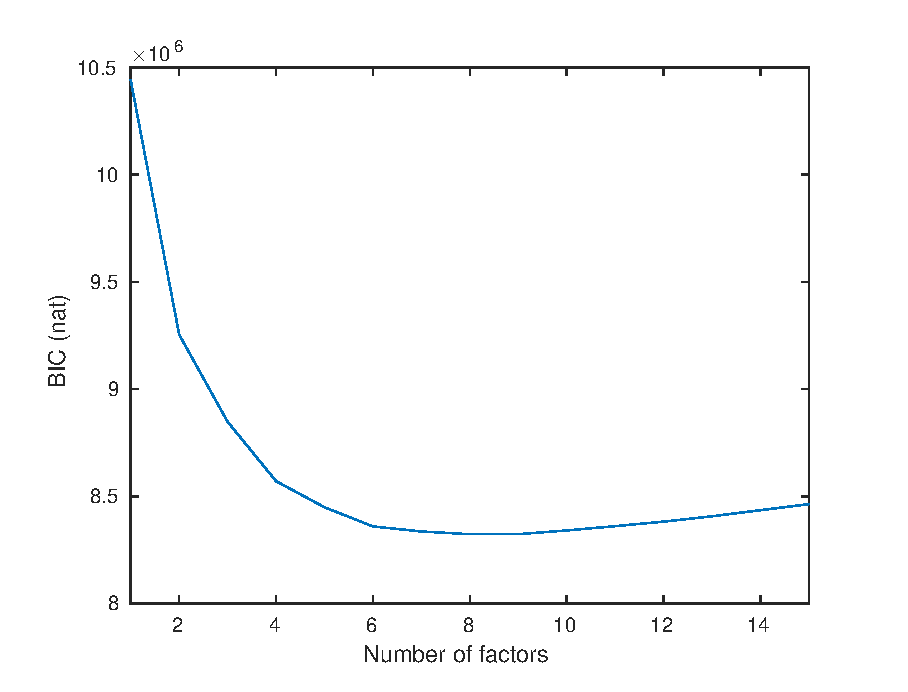
\includegraphics[width=\textwidth]{figures/initial_factor_BIC.eps}
	\caption{BIC for fitting different number of factors onto the data. 81 different initials were used for each $k$ with a stopping condition of 100 EM steps.}
	\label{fig:initial_factor_BIC}
\end{figure}

\begin{figure}
	\centering
	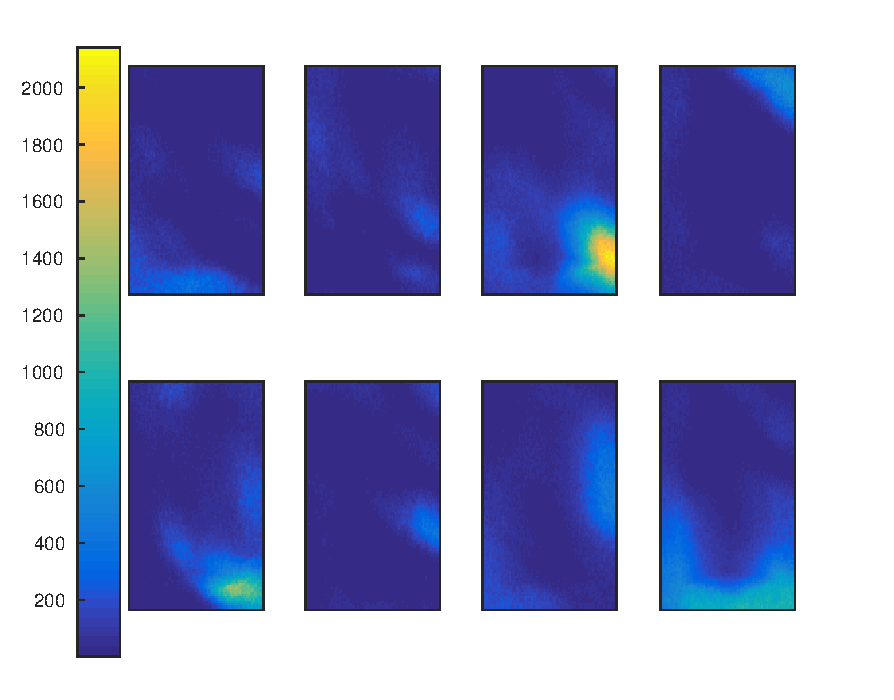
\includegraphics[width=\textwidth]{figures/initial_factor_factorNoise.eps}
	\caption{The 8 individual factor variances with the lowest log likelihood found.}
	\label{fig:initial_factor_factorNoise}
\end{figure}

\begin{figure}
	\centering
	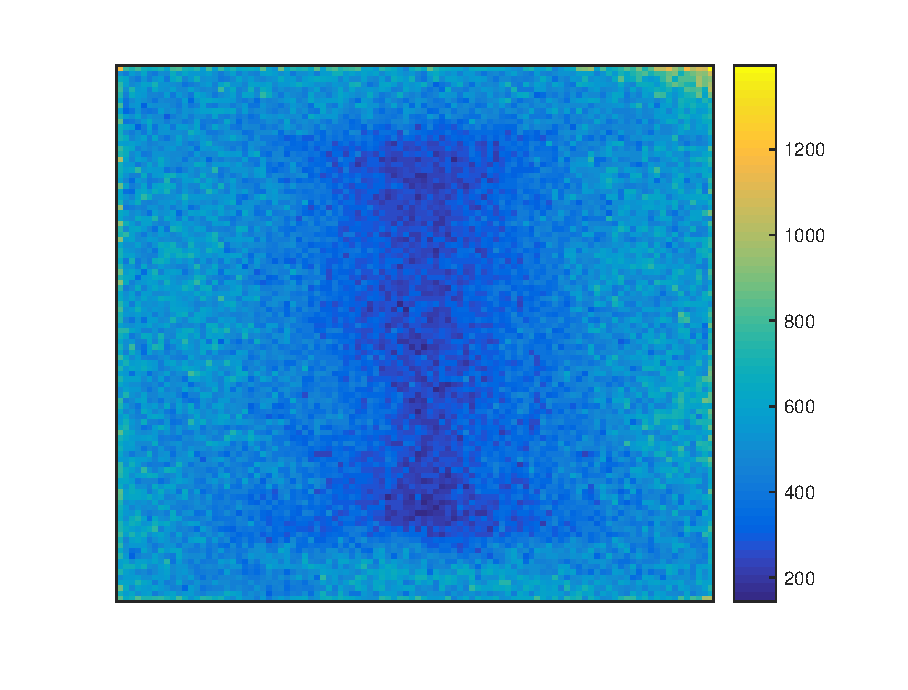
\includegraphics[width=\textwidth]{figures/initial_factor_instrinicNoise.eps}
	\caption{The intrinsic variances with the lowest log likelihood found.}
	\label{fig:initial_factor_instrinicNoise}
\end{figure}

The uncertainty of model selection was assessed by investigating how the BIC and optimal $k$ varied for different bootstrap samples. The BIC for the 99 bootstrap samples is shown in Figure \ref{fig:initial_factor_BIC_bootstrap}. Only one initial value was used for each $k$ to capture the uncertainty if the EM algorithm converges to a global maxima or not. From the figure, quite clearly there was a lot of variability in the BIC and can cause imprecise decisions on model selection. Over all 99 bootstrap samples, the mean and standard deviation optimal $k$ was found to be $10\pm2$ factors.

The main source of error was down to the small sample size. The experiments can be improved if the analysis was done on the full size image rather than downsizing it. When downsizing, there is a risk of tampering the variance of the pixel's grey values.

\begin{figure}
	\centering
	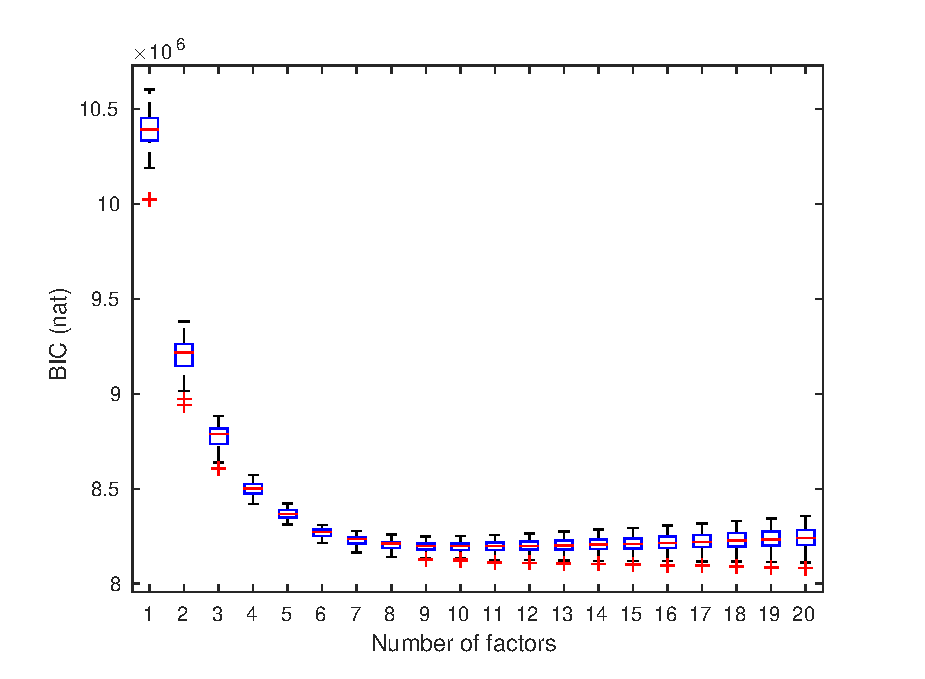
\includegraphics[width=\textwidth]{figures/initial_factor_BIC_bootstrap.eps}
	\caption{BIC for fitting different number of factors onto the data. 99 bootstrap samples were used and only 1 initial value was used for each $k$. A stopping condition of 100 EM steps was used.}
	\label{fig:initial_factor_BIC_bootstrap}
\end{figure}

\chapter{Mean and Variance Relationship}
The aim of this chapter was to do supervised learning on predicting the variance of the pixel's grey values given its mean. By training a classifier, a single CT scan can be used to quantify the uncertainty on each pixel's grey values. This uncertainty is then carried forward when doing volumetric reconstruction.

\section{Weighted Least Squares}
\subsection{Theory}
The sample variance of the grey values is a random variable, thus has variance or in other words uncertainty. Weighted least squares can be used to take into consideration the uncertainty of the sample variance. This can be done by giving low weights to data points with high uncertainty on the grey value variance.

Let $S_i^2$ and $\sigma_i^2$ be the sample variance and true variance, respectively, of the $i$th pixel's grey value for $i=1,2,\dotdotdot,m$. The sample variance has a sampling distribution such that
\begin{equation}
U_i=\frac{(n-1)S_i^2}{\sigma_i^2}\sim\chi_{n-1}^2
\end{equation}
where $n$ is the number of samples used in estimating the variance. The variance is then
\begin{equation}
2(n-1)=\frac{(n-1)^2}{\sigma_i^4}\variance\left(S_i^2\right)
\end{equation}
thus
\begin{equation}
\variance\left(S_i^2\right)=\frac{2\sigma_i^4}{n-1} \ .
\end{equation}

A good weight for pixel $i$, $w_i$, would be one which is proportional to the precision, or reciprocal of the variance, of $S_i^2$. $\sigma_i^2$ is generally unknown but can be estimated using $S_i^2$. By doing so, the weights for each grey value was chosen to be
\begin{equation}
w_i \propto \frac{1}{\left(S_i^2\right)^2} \ .
\end{equation}

The weights can be introduced into the least squares problem.  Let $Y_1,Y_2,\dotdotdot,Y_m$ be the sample variance of the grey values and $\vect{x}_1,\vect{x}_2,\dotdotdot,\vect{x}_m$ be the feature vectors of the sample mean of the grey values. The weighted least squares is an optimization problem where the objective is
\begin{equation}
T =
\frac{\sum_{i=1}^mw_i\left(Y_i-\left(\vect{x}_i\right)\T\vectGreek{\beta}\right)^2}
{\sum_{i=1}^mw_i} \ .
\end{equation}
This can be expanded
\begin{equation}
T =
\frac{\sum_{i=1}^mw_i\left(Y_i-2Y_i\vectGreek{\beta}\T\vect{x}_i+\vectGreek{\beta}\T\vect{x}_i\left(\vect{x}_i\right)\T\vectGreek{\beta}\right)}
{\sum_{i=1}^mw_i} \ .
\end{equation}
Using the properties of the trace
\begin{equation}
T =
\frac{\sum_{i=1}^mw_i\left(Y_i-2Y_i\trace\left(\vectGreek{\beta}\T\vect{x}_i\right)+\trace\left(\vectGreek{\beta}\T\vect{x}_i\left(\vect{x}_i\right)\T\vectGreek{\beta}\right)\right)}
{\sum_{i=1}^mw_i}
\end{equation}
the differential with respect to $\vectGreek{\beta}$ is
\begin{equation}
\nabla_{\vectGreek{\beta}}T = \frac{-2\sum_{i=1}^mw_iY_i\vect{x}_i+2\sum_{i=1}^mw_i\vect{x}_i\left(\vect{x}_i\right)\T\vectGreek{\beta}}{\sum_{i=1}^mw_i} \ .
\end{equation}
Setting the differential to 0
\begin{equation}
\vectGreek{\beta}=\left[\sum_{i=1}^mw_i\vect{x}_i\left(\vect{x}_i\right)\T\right]^{-1}\sum_{i=1}^mw_i\vect{x}_iY_i \ .
\end{equation}

Assuming $Y_1,Y_2,\dotdotdot,Y_m$ are independent and have constant variance $\sigma^2$, the covariance of the weighted least squares is
\begin{equation}
\cov(\vectGreek{\beta})=
\sigma^2\left[\sum_{i=1}^mw_i\vect{x}_i\left(\vect{x}_i\right)\T\right]^{-1}\left[\sum_{i=1}^mw_i\vect{x}_i\right]\left[\sum_{i=1}^mw_i\left(\vect{x}_i\right)\T\right]\left[\sum_{i=1}^mw_i\vect{x}_i\left(\vect{x}_i\right)\T\right]^{-1} \ .
\end{equation}

$\sigma^2$ can be estimated using the weighted mean squared error
\begin{equation}
\widehat{\sigma}^2=\frac{\sum_{i=1}^mw_i\left[Y_i-\left(\vect{x}_i\right)\T\vectGreek{\beta}\right]^2}{\sum_{i=1}^mw_i} \ .
\end{equation}

After estimating $\vectGreek{\beta}$ and $\sigma^2$ and given a data point $\vect{x}_{\textup{test}}$, then the predicted variance is
\begin{equation}
\widehat{Y}=\left(\vect{x}_{\textup{test}}\right)\T\vectGreek{\beta} + \epsilon_{\textup{test}}
\end{equation}
with expectation
\begin{equation}
\expectation\left({\widehat{Y}}\right)=\left(\vect{x}_{\textup{test}}\right)\T\vectGreek{\beta}
\end{equation}
and variance
\begin{equation}
\variance\left(\widehat{Y}\right)=\left(\vect{x}_{\textup{test}}\right)\T\cov(\vectGreek{\beta})\vect{x}_{\textup{test}}+\sigma^2 \ .
\end{equation}

\subsection{Methods}
The sample mean and sample variance were calculated for all 3\,984\,016 pixel's grey values. Polynomial features were constructed, up to order $k$, using the sample mean. The weighted linear regression was then fitted.

Before fitting the linear regression, the weighted were normalized to have a maximum of 1. Furthermore, each feature was normalized to have mean 0 and standard deviation 1. Afterwards, a constant of 1 was appended to the feature vector to model the intercept of the linear regression.

As in previous experiments, the BIC was used to do model selection.

\subsection{Results}
The weighted least squares with polynomial features were fitted successfully as shown in Figure \ref{fig:weightedLS_polynomials}. It can be observed that the weighted least squares gave less weights to data points with high sample variance, thus in a way treating them like outliers.

The BIC, as shown in Figure \ref{fig:weightedLS_BIC}, favoured high order polynomials. Because the BIC favoured more complicated models, this suggested that fitting polynomial features was not a good model. The BIC aimed to seek more and more polynomials so that the model become more similar to the true model. 

\begin{figure}
	\centering
	\begin{subfigure}{0.45\textwidth}
		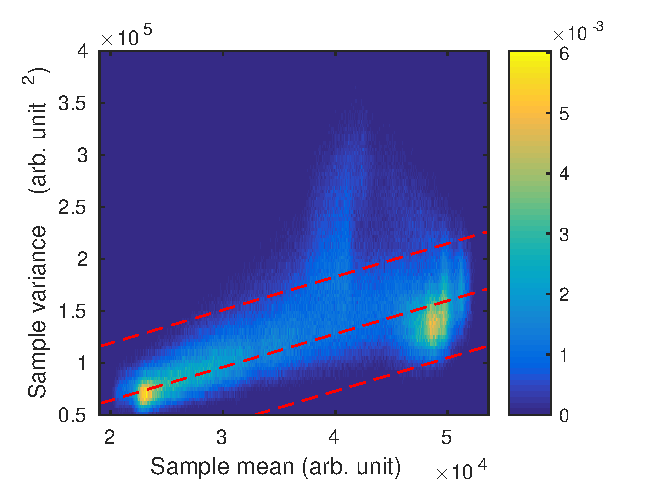
\includegraphics[width=\textwidth]{figures/meanVar/order1.eps}
		\caption{Order 1}
	\end{subfigure}
	\begin{subfigure}{0.45\textwidth}
		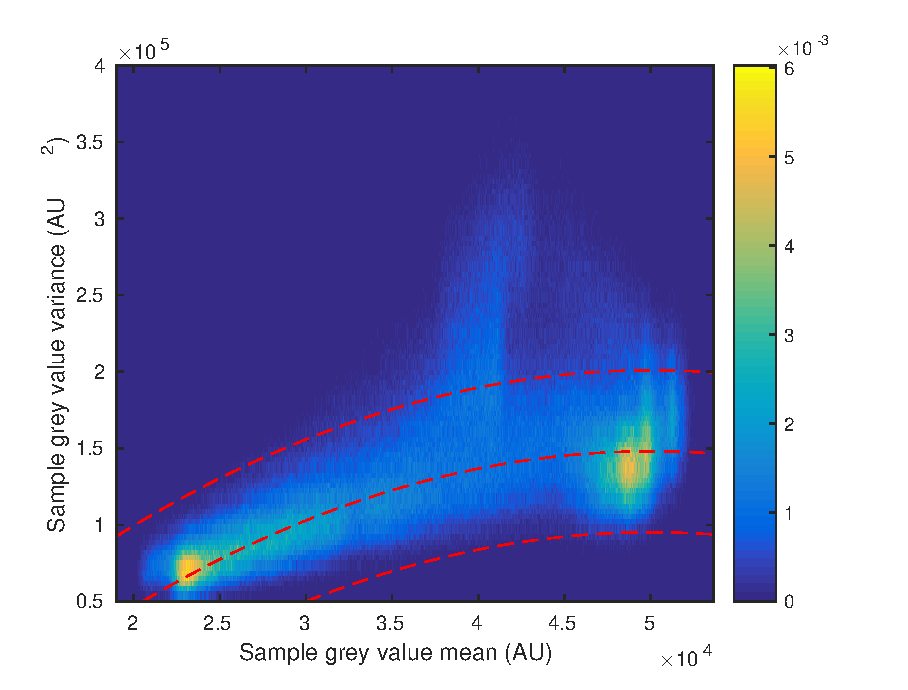
\includegraphics[width=\textwidth]{figures/meanVar/order2.eps}
		\caption{Order 2}
	\end{subfigure}
	\begin{subfigure}{0.45\textwidth}
		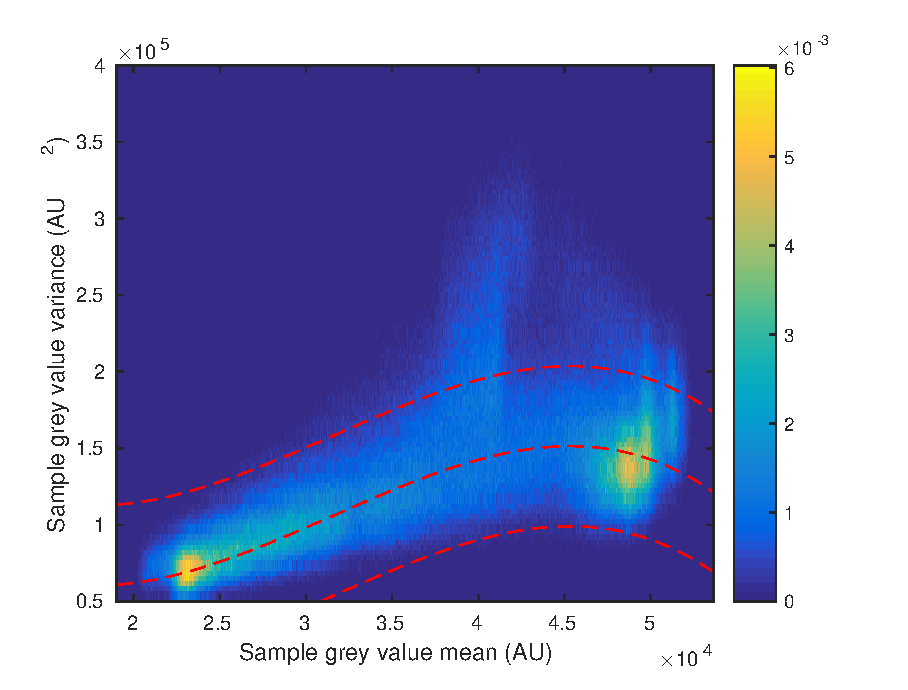
\includegraphics[width=\textwidth]{figures/meanVar/order3.eps}
		\caption{Order 3}
	\end{subfigure}
	\begin{subfigure}{0.45\textwidth}
		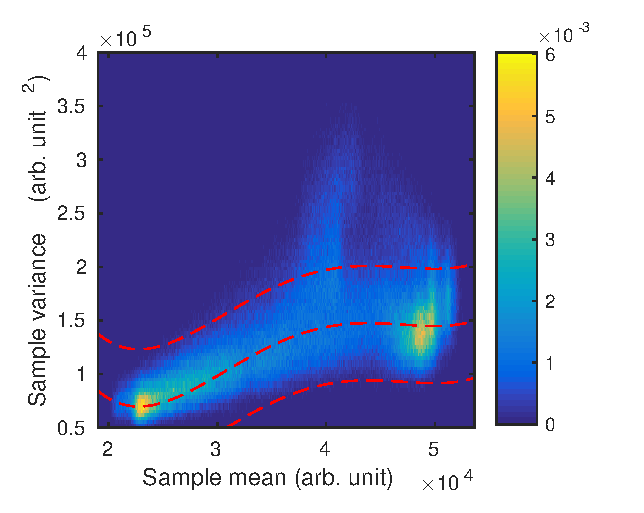
\includegraphics[width=\textwidth]{figures/meanVar/order4.eps}
		\caption{Order 4}
	\end{subfigure}
	\begin{subfigure}{0.45\textwidth}
		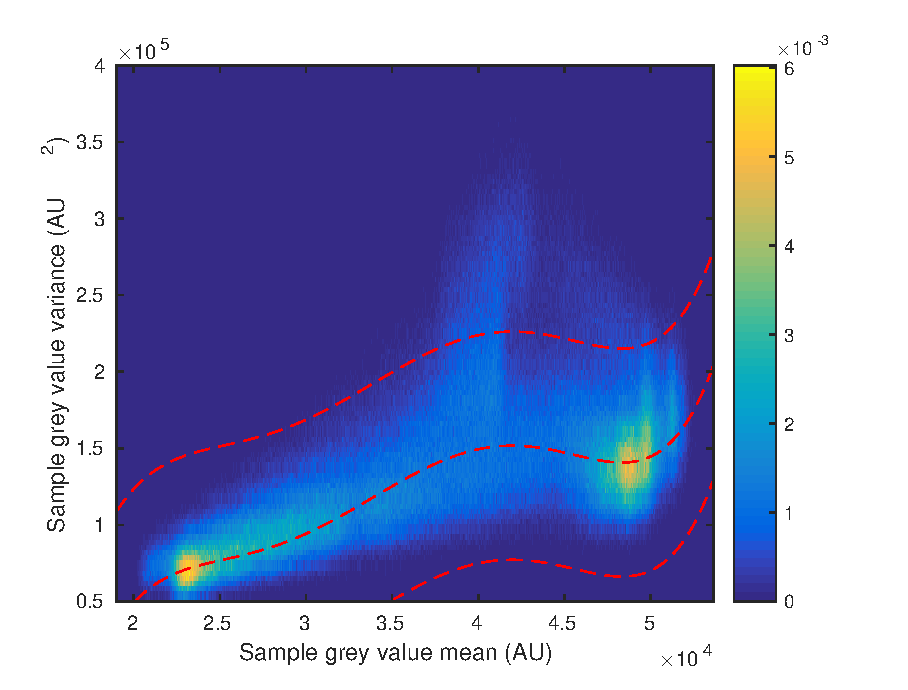
\includegraphics[width=\textwidth]{figures/meanVar/order5.eps}
		\caption{Order 5}
	\end{subfigure}
	\begin{subfigure}{0.45\textwidth}
		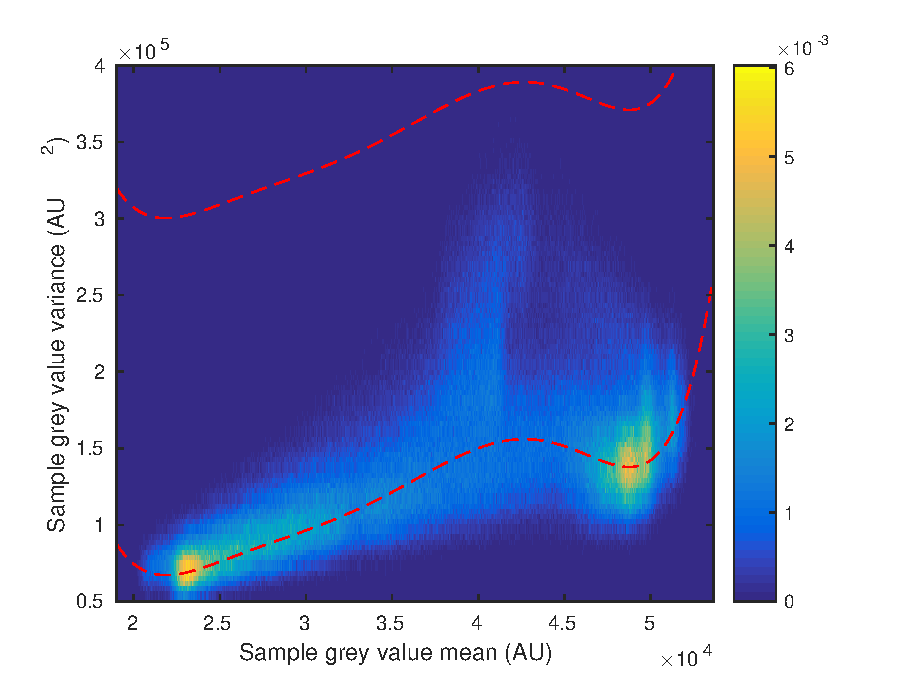
\includegraphics[width=\textwidth]{figures/meanVar/order6.eps}
		\caption{Order 6}
	\end{subfigure}
	\caption{Frequency density plots of the sample mean and variance of the grey values. Weighted least squares with polynomial features was fitted. The (red) dotted line represent the 95\% prediction interval.}
	\label{fig:weightedLS_polynomials}
\end{figure}

\begin{figure}
	\centering
	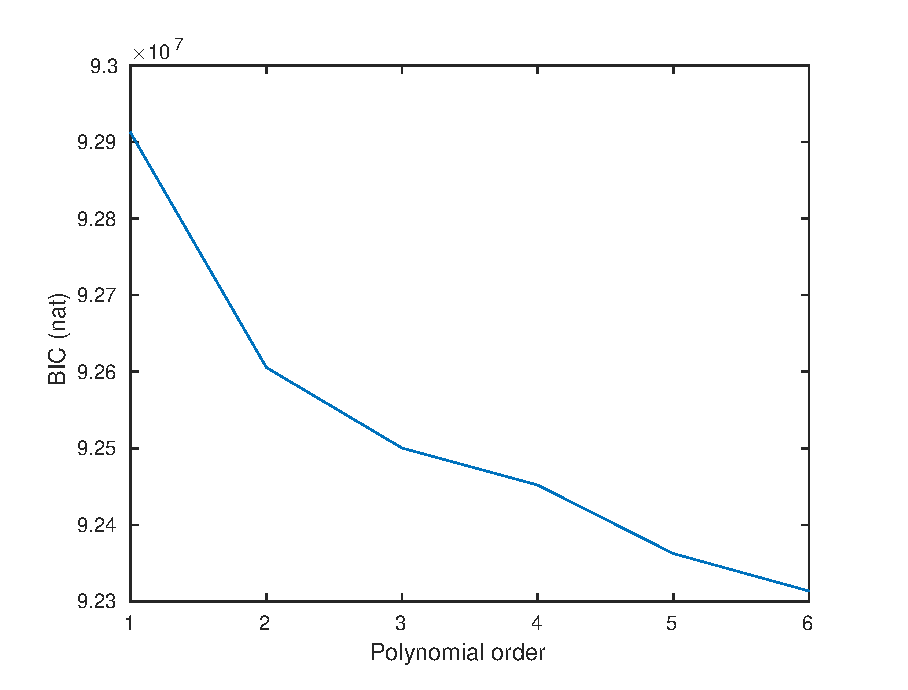
\includegraphics[width=0.6\textwidth]{figures/meanVar/polynomialBIC.eps}
	\caption{Weighted BIC when for fitting weighted least squares with polynomial features on the sample mean sample variance pairs.}
	\label{fig:weightedLS_BIC}
\end{figure}

\section{Subsampling Least Squares}
\subsection{Methods}
From the previous chapter, it was clear there were 3 materials, the sample, background and foam, which contributed to the peaks in the histogram of the grey values.

The sample mean sample variance pairs were sub-sampled from each of the 3 materials. A 1st order linear regression was fitted for each sub-sample.

\subsection{Results}

It is clear the gradients are material dependent.

\begin{figure}
	\centering
	\begin{subfigure}{0.45\textwidth}
		\includegraphics[width=\textwidth]{figures/meanVar/subsample_sample.eps}
		\caption{Sample}
	\end{subfigure}
	\begin{subfigure}{0.45\textwidth}
		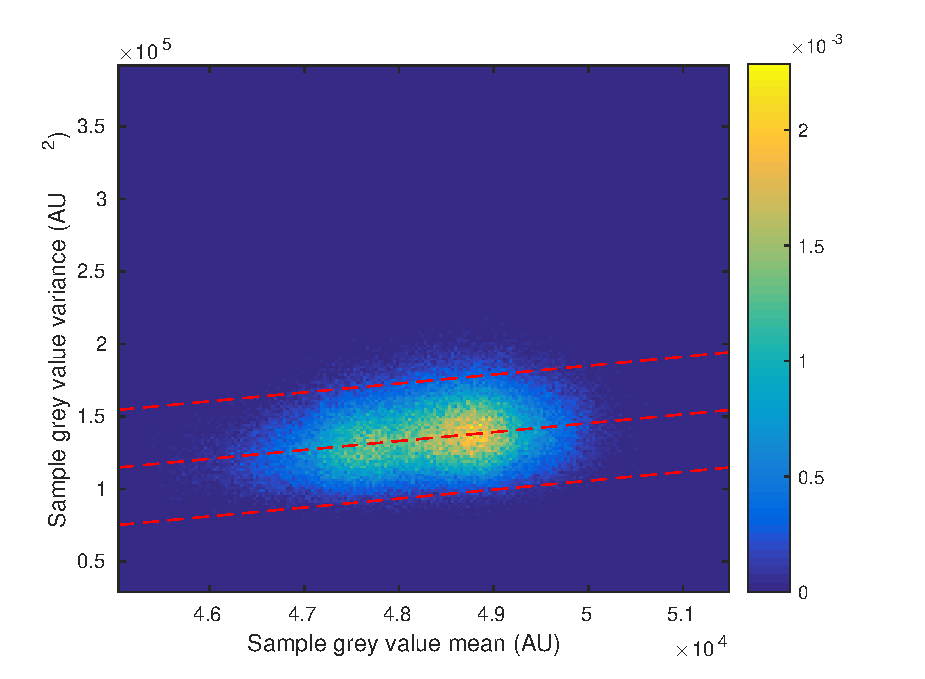
\includegraphics[width=\textwidth]{figures/meanVar/subsample_background.eps}
		\caption{Background}
	\end{subfigure}
	\begin{subfigure}{0.45\textwidth}
		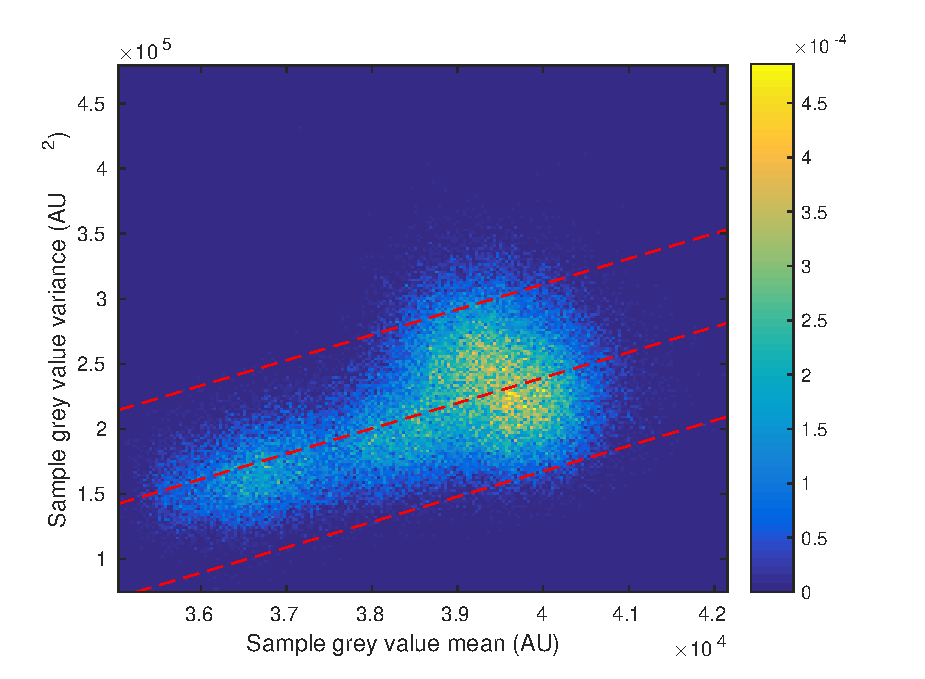
\includegraphics[width=\textwidth]{figures/meanVar/subsample_foam.eps}
		\caption{Foam}
	\end{subfigure}
	\caption{A linear regression was fitted on a subsample of sample mean-variance pairs for each material.}
\end{figure}

\begin{figure}
	\centering
	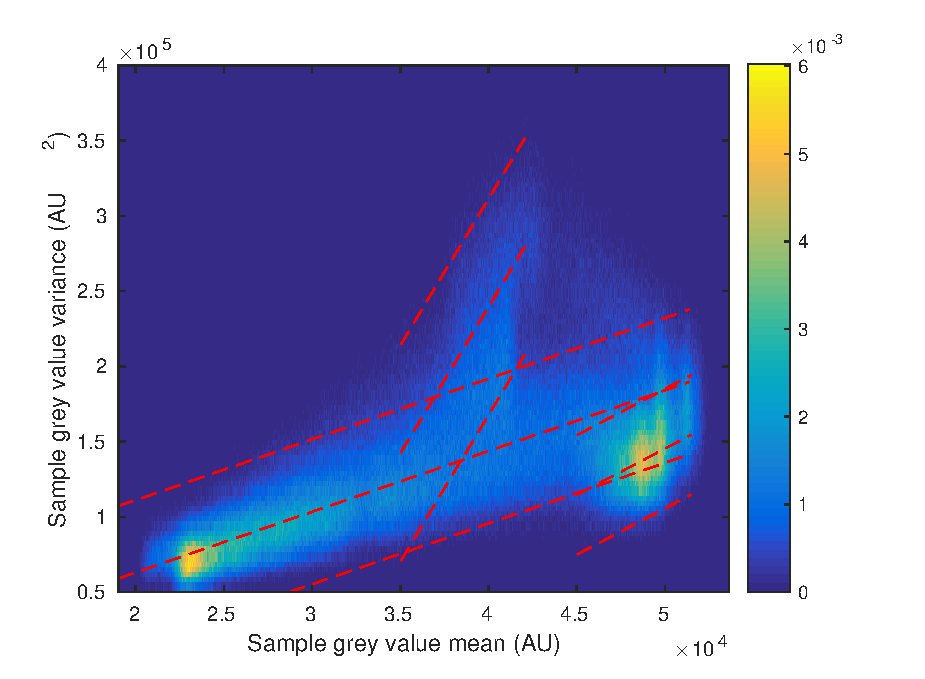
\includegraphics[width=0.6\textwidth]{figures/meanVar/subsample.eps}
	\caption{Frequency density of all the sample mean-variance pairs. The dotted lines represent the 95\% prediction interval of the least squares regression for each sub-sample, these lines ranges so that they do not extrapolate.} 
\end{figure}

\section{Mixture of Linear Regression}
\subsection{Theory}
In order to consider the 3 different materials, a mixture of linear regression was used of the form
\begin{equation}
Y_i\sim
\begin{cases}
\normal\left(\left(\vect{x}_i\right)\T\vectGreek{\beta}_1,\sigma_1^2\right) & \text{if }S_i=1\\ 
\normal\left(\left(\vect{x}_i\right)\T\vectGreek{\beta}_2,\sigma_2^2\right) & \text{if }S_i=2\\ 
\normal\left(\left(\vect{x}_i\right)\T\vectGreek{\beta}_3,\sigma_3^2\right) & \text{if }S_i=3\\
\end{cases}
\end{equation}
where $S_i$ is a latent variable and $\prob\left(S_i=r\right)=\pi_r$ for $i=1,2,\dotdotdot,m$.

The likelihood is
\begin{equation}
L=\prod_{i=1}^m\sum_{j=1}^3p_{Y|S}\left(y_i|S_i=j\right)\pi_j
\end{equation}
thus the log likelihood is
\begin{equation}
\ln{L}=\sum_{i=1}^m\ln\left[
\sum_{j=1}^3p_{Y|S}\left(y_i|S_i=j\right)\pi_j
\right] \ .
\end{equation}
Such a log likelihood can be maximised by using the EM algorithm, treating $S_i$ as a random latent variable.

In the E step, the posterior distribution is used to put a distribution on $S_i$ for $i=1,2,\dotdotdot,m$ given the parameters $\vectGreek{\beta}_j$, $\sigma_j^2$ and $\pi_j$ for $j=1,2,3$. The posterior distribution is given as
\begin{equation}
r_{i,j}=\prob\left(S_i=j|Y_i=y_i\right)=\frac
{p_{Y|S}\left(y_i|S_i=j\right)\pi_j}
{\sum_{j'=1}^3p_{Y|S}\left(y_i|S_i=j'\right)\pi_j}
\end{equation}
and just a quantity is called the responsibility of the $i$th data belonging to the $j$th model.

In the M step, the parameters $\vectGreek{\beta}_j$, $\sigma_j^2$ and $\pi_j$ for $j=1,2,3$ are updated given the posterior distribution of $S_i$ for $i=1,2,\dotdotdot,m$. Consider some arbitrary parameter $\theta_j$ which model $j$ depends on. Then
\begin{equation}
\frac{\partial\ln{L}}{\partial\theta_j}=
\sum_{i=1}^m\frac{\pi_j}{\sum_{j'=1}^3p_{Y|S}\left(y_i|S_i=j'\right)\pi_j}
\frac{\partial p_{Y|S}\left(y_i|S_i=j\right)}{\partial\theta_j}
\end{equation}
\begin{equation}
\frac{\partial\ln{L}}{\partial\theta_j}=
\sum_{i=1}^m\frac{p_{Y|S}\left(y_i|S_i=j\right)\pi_j}{\sum_{j'=1}^3p_{Y|S}\left(y_i|S_i=j'\right)\pi_j}
\frac{\partial \ln\left[p_{Y|S}\left(y_i|S_i=j\right)\right]}{\partial\theta_j}
\end{equation}
which is just
\begin{equation}
\frac{\partial\ln{L}}{\partial\theta_j}=
\sum_{i=1}^mr_{i,j}
\frac{\partial \ln\left[p_{Y|S}\left(y_i|S_i=j\right)\right]}{\partial\theta_j} \ .
\end{equation}
Using the above result
\begin{equation}
\nabla_{\vectGreek{\beta}_j}\ln{L}
=\sum_{i=1}^{m}
r_{i,j}
\nabla_{\vectGreek{\beta}_j}
\ln\left[
	\frac{1}{\sqrt{2\pi}\sigma_j}\exp\left(-\frac{1}{2}\left(\frac{y_i-\left(\vect{x}_i\right)\T\vectGreek{\beta}_j}{\sigma_j}\right)^2\right)
\right]
\end{equation}
\begin{equation}
\nabla_{\vectGreek{\beta}_j}\ln{L}
=\sum_{i=1}^{m}
r_{i,j}
\nabla_{\vectGreek{\beta}_j}
\left[
	-\frac{1}{2}\ln(2\pi) - \frac{1}{2}\ln\left(\sigma_j^2\right)-\frac{1}{2}\left(\frac{y_i-\left(\vect{x}_i\right)\T\vectGreek{\beta}_j}{\sigma_j}\right)^2
\right] \ .
\end{equation}
Expanding it out
\begin{equation}
\nabla_{\vectGreek{\beta}_j}\ln{L}
=\sum_{i=1}^{m}
r_{i,j}
\nabla_{\vectGreek{\beta}_j}
\left[-\frac{1}{2\sigma_j^2}\left(-2y_i\vectGreek{\beta}_j\T\vect{x}_i
+\vectGreek{\beta}_j\T\vect{x}_i\left(\vect{x}_i\right)\T\vectGreek{\beta}_j
\right)
+c_1
\right]
\end{equation}
and using the properties of the trace
\begin{equation}
\nabla_{\vectGreek{\beta}_j}\ln{L}
=\sum_{i=1}^{m}
r_{i,j}
\nabla_{\vectGreek{\beta}_j}
\left[-\frac{1}{2\sigma_j^2}\left(-2y_i\trace\left(\vectGreek{\beta}_j\T\vect{x}_i\right)
+\trace\left(\vectGreek{\beta}_j\T\vect{x}_i\left(\vect{x}_i\right)\T\vectGreek{\beta}_j
\right)\right)
+c_1
\right]
\end{equation}
\begin{equation}
\nabla_{\vectGreek{\beta}_j}\ln{L}
=\sum_{i=1}^{m}
-\frac{r_{i,j}}{2\sigma_j^2}
\left(-2y_i\vect{x}_i
+2\vect{x}_i\left(\vect{x}_i\right)\T\vectGreek{\beta}_j
\right) \ .
\end{equation}
Setting this to zero
\begin{equation}
\sum_{i=1}^{m}
r_{i,j}
y_i\vect{x}_i
=
\sum_{i=1}^{m}r_{i,j}
\vect{x}_i\left(\vect{x}_i\right)\T\vectGreek{\beta}_j
\end{equation}
\begin{equation}
\vectGreek{\beta}_j
=
\left[\sum_{i=1}^{m}r_{i,j}
\vect{x}_i\left(\vect{x}_i\right)\T\right]^{-1}
\left[\sum_{i=1}^{m}
r_{i,j}
y_i\vect{x}_i\right]
\end{equation}
and this is just weighted least squares where the weights are the responsibilities on model $j$.

By re-parametrise $1/\sigma_j^2=\tau_j$
\begin{equation}
\frac{\partial\ln{L}}{\partial\tau_j}
=\sum_{i=1}^{m}
r_{i,j}
\frac{\partial}{\partial\tau_j}
\left[
	-\frac{1}{2}\ln(2\pi) + \frac{1}{2}\ln\left(\tau_j\right)-\frac{\tau_j}{2}\left({y_i-\left(\vect{x}_i\right)\T\vectGreek{\beta}_j}\right)^2
\right]
\end{equation}
\begin{equation}
\frac{\partial\ln{L}}{\partial\tau_j}
=\sum_{i=1}^{m}
r_{i,j}
\left[\frac{1}{2\tau_j}-\frac{1}{2}\left({y_i-\left(\vect{x}_i\right)\T\vectGreek{\beta}_j}\right)^2
\right] \ .
\end{equation}
Setting this to zero
\begin{equation}
\sigma_j^2
=
\frac{\sum_{i=1}^{m}
r_{i,j}\left({y_i-\left(\vect{x}_i\right)\T\vectGreek{\beta}_j}\right)^2}
{\sum_{i=1}^{m}r_{i,j}}
\end{equation}
and this is just the weighted mean squared error.

To obtain the maximum log likelihood estimator for $\pi_j$, a Lagrange multiplier must be used to put a constraint that $\sum_{j=1}^3\pi_j=1$. The objective is then
\begin{equation}
T = \ln{L} + \lambda\left(\sum_{j=1}^3\pi_j-1\right)
\end{equation}
\begin{equation}
\frac{\partial T}{\partial\pi_j}=\frac{\partial}{\partial\pi_j}\sum_{i=1}^m\ln\left[
\sum_{j'=1}^3p_{Y|S}\left(y_i|S_i=j'\right)\pi_{j'}
\right] + \lambda
\end{equation}
\begin{equation}
\frac{\partial T}{\partial\pi_j}=\sum_{i=1}^m\frac{p_{Y|S}\left(y_i|S_i=j\right)}{\sum_{j'=1}^3p_{Y|S}\left(y_i|S_i=j'\right)\pi_{j'}} + \lambda
\end{equation}
\begin{equation}
\frac{\partial T}{\partial\pi_j}=\sum_{i=1}^m\frac{r_{i,j}}{\pi_j} + \lambda \ .
\end{equation}
Setting this to zero
\begin{equation}
\pi_j = \sum_{i=1}^m\frac{r_{i,j}}{\lambda} \ .
\end{equation}
$\lambda$ can be determined by putting a constraint on the estimators of $\pi_j$ for $j=1,2,3$
\begin{equation}
\sum_{j=1}^3\sum_{i=1}^m\frac{r_{i,j}}{\lambda}=1
\end{equation}
\begin{equation}
\sum_{i=1}^m\sum_{j=1}^3r_{i,j}=\lambda
\end{equation}
\begin{equation}
\sum_{i=1}^m1=\lambda
\end{equation}
\begin{equation}
m=\lambda
\end{equation}
therefore
\begin{equation}
\pi_j = \sum_{i=1}^m\frac{r_{i,j}}{m} \ .
\end{equation}
This is the average responsibility.

All steps in the EM algorithm have been derived.

\subsection{Methods}
The EM algorithm was initialised by assigning random responsibilities for all models and data points in the E step.

\subsection{Results}
It was verified that the EM algorithm always increased the log likelihood at every EM step, as can be seen in Figure \ref{fig:mixture_lnL}.

The resulting fit, as shown in Figure \ref{fig:mixture_histogram}, did not capture the 3 different materials. This is because the mixture probabilities, $\pi_1,\pi_2,\pi_3$, do not depend on the sample-mean of the grey values. For example, low grey values are more likely to be from the sample.

\begin{figure}
	\centering	
	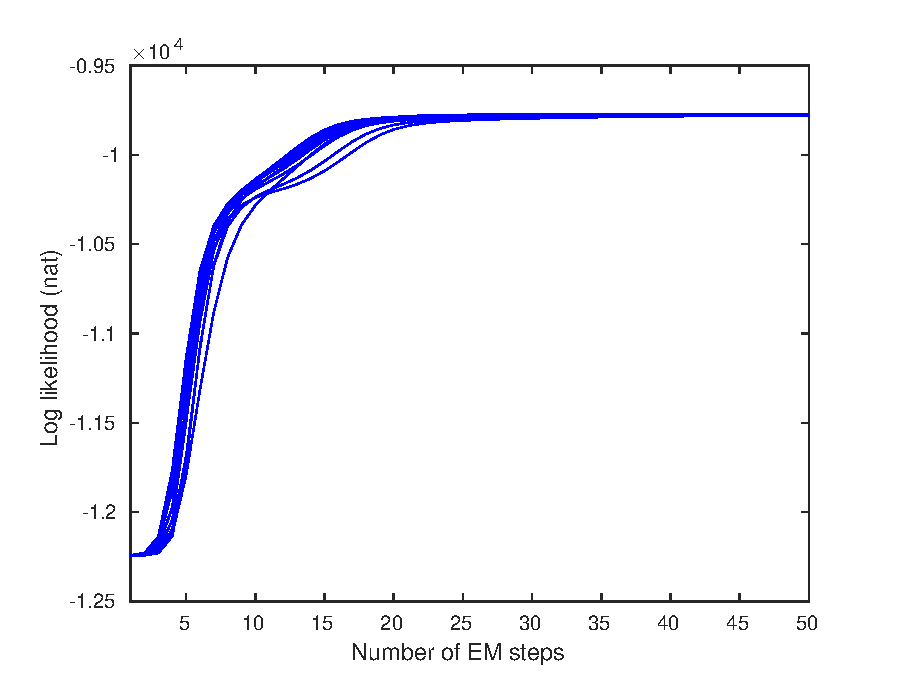
\includegraphics[width=0.6\textwidth]{figures/meanVar/mixture_lnL.eps}
	\caption{The log likelihood of the mixture of linear regressions at every EM step for 10 different initial values.}
	\label{fig:mixture_lnL}
\end{figure}

\begin{figure}
	\centering	
	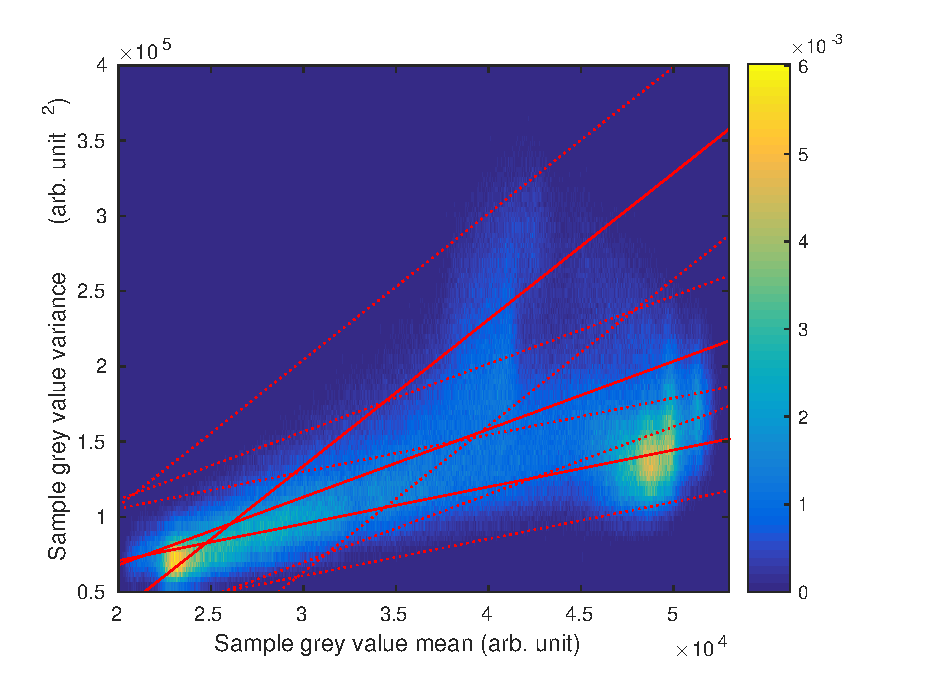
\includegraphics[width=0.6\textwidth]{figures/meanVar/mixture_histogram.eps}
	\caption{Fitting a mixture of 3 linear regressions on the sample mean-variance data.}
	\label{fig:mixture_histogram}
\end{figure}

\section{Distance Weighted Least Squares}
\subsection{Methods}
To consider the 3 different sources, weighted least squares can be used where the weights depends on some distance from some particular sample-mean grey value. 3 different weighted least squares were used where the weights are
\begin{equation}
w_i\propto\exp\left[-\frac{1}{2}\left(\frac{x_i-\mu_j}{\sigma_j}\right)^2\right]
\end{equation}
$\mu_j$ was found using $k$-means in the sample-mean grey value space and $\sigma_j$ is predefined constant, called the Gaussian width.
\subsection{Results}

The model captured the sample and foam well because the regression captured the shape of the histogram. However for the background, the regression can be negative as a result of being influenced by lower sample grey values from the foam and sample.

For higher Gaussian widths, the regression becomes an ordinary least squares regression because all the data points approximately equal weights.

\begin{figure}
	\centering
	\begin{subfigure}{0.45\textwidth}
		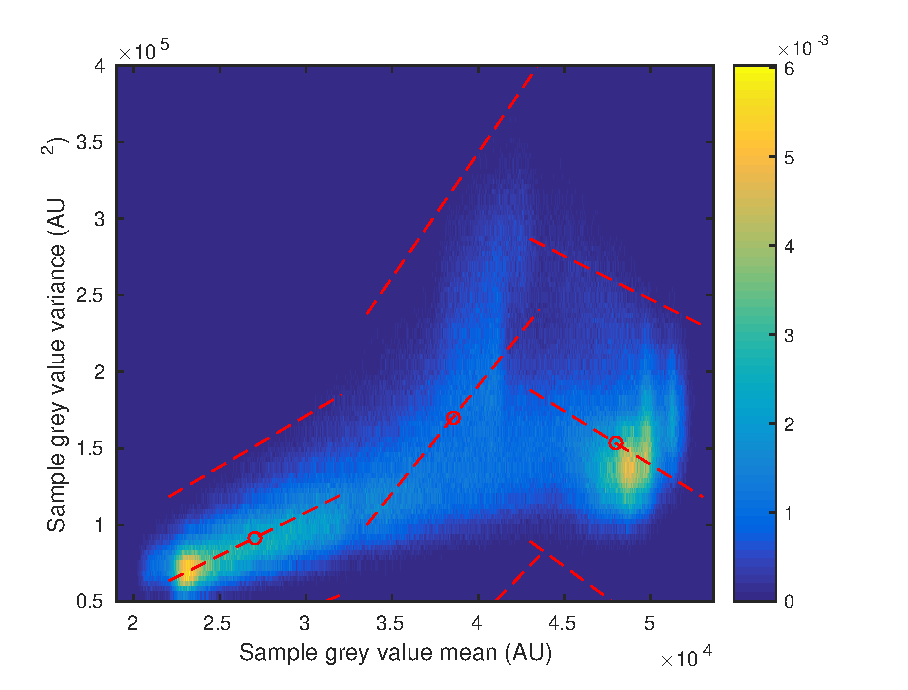
\includegraphics[width=\textwidth]{figures/meanVar/gaussian_1.eps}
		\caption{$\sigma=10^2$}
	\end{subfigure}
	\begin{subfigure}{0.45\textwidth}
		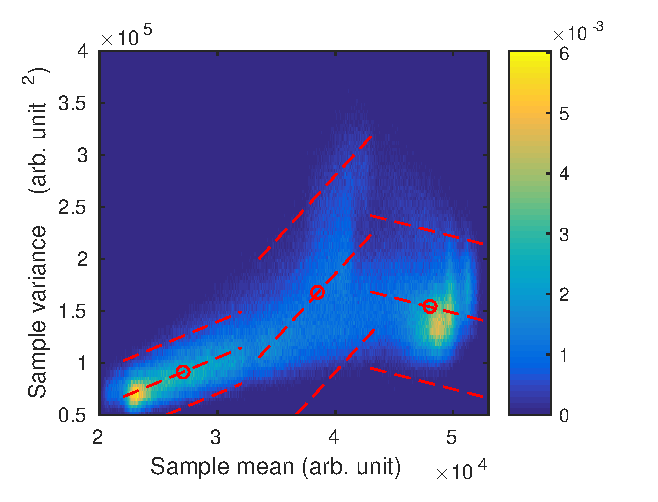
\includegraphics[width=\textwidth]{figures/meanVar/gaussian_2.eps}
		\caption{$\sigma=10^3$}
	\end{subfigure}
	\begin{subfigure}{0.45\textwidth}
		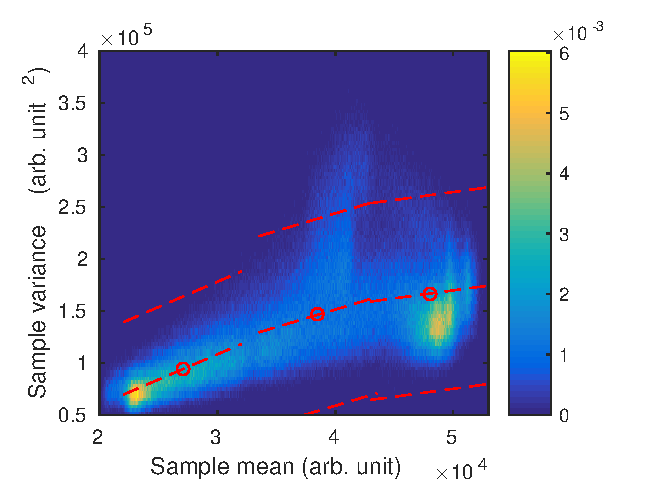
\includegraphics[width=\textwidth]{figures/meanVar/gaussian_3.eps}
		\caption{$\sigma=10^4$}
	\end{subfigure}
	\begin{subfigure}{0.45\textwidth}
		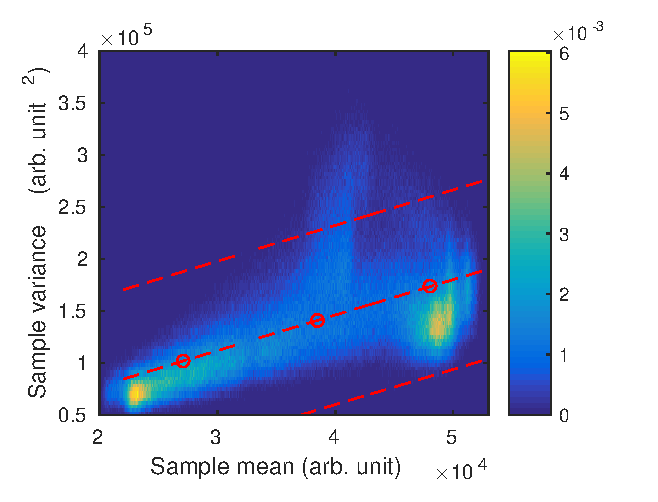
\includegraphics[width=\textwidth]{figures/meanVar/gaussian_4.eps}
		\caption{$\sigma=10^5$}
	\end{subfigure}
	\caption{3 independent Gaussian weighted least squares regressions. The weights depend on the distance from the $k$-means sample mean grey values and some width $\sigma$.}
\end{figure}

\chapter{Model for Intensity}
\section{Rate Density}
Consider photons emitted from an X-ray tube. These photons have a board energy spectrum as a result of Bremsstrahlung and characteristic radiation. An experiment can be conducted by measuring the energy of each photon, over some exposure time, to obtain a histogram of photon energies, similar to the one in Figure \ref{fig:x_ray_spectrum2}.

\begin{figure}
\centering
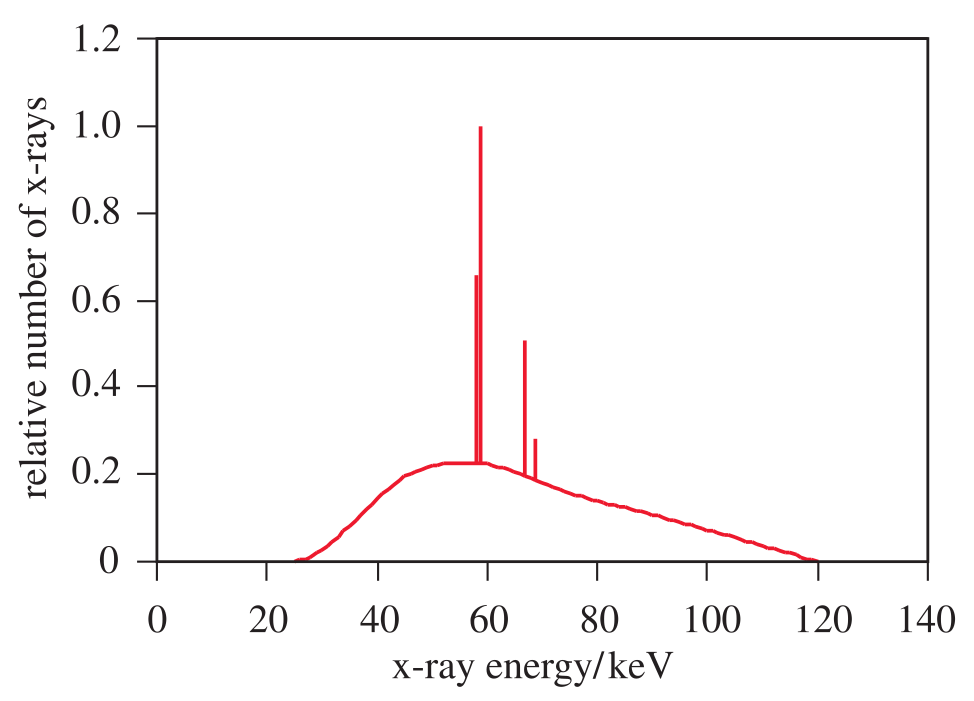
\includegraphics[width=0.8\textwidth]{figures/x_ray_spectrum.png}
\caption{A typical energy spectrum of X-ray photons emitted from an X-ray tube. The continuous spectrum is the result of Bremmsstrahlung radiation. The peaks are the result of characteristic radiation. \emph{Source: G.~Michael (2001) \cite{michael2001x}}}
\label{fig:x_ray_spectrum2}
\end{figure}

In order to model the number of photons detected in some exposure time as a Poisson process, the rate of photons emitted is an important variable. However it is nonsense to talk about the rate of photons with energy exactly $E$. This is because energy is a continuous variable and cannot be modelled discretely. Instead the rate of photons with energy $E_1<E<E_2$ should be considered.

To take into consideration the continuous nature of energy, the histogram of photon energies should be normalised in such a way that the area of the histogram is the rate of photons, with any energy, detected. This will produce an approximation to the rate density function $\lambda(E)$. The rate density function has units of $\textup{s}^{-1}\cdot\textup{keV}^{-1}$.

The rate density function has the following properties.
\begin{equation}
\text{rate of photons with energy }E_1<E<E_2=
\int_{E_1}^{E_2}\lambda(E)\diff E
\end{equation}
\begin{equation}
\text{rate of photons with any energy }=
\int_{0}^{\infty}\lambda(E)\diff E
\end{equation}

The expected energy can be calculated by splitting the rate density function into $n$ equal intervals, of size $\Delta E$, $E_1,E_2,\dotdotdot,E_n$. A weighted mean can be used to estimate the expected energy
\begin{equation}
\expectation[E]=\frac{\sum_{i=1}^nE_i\lambda(E_i)\Delta E}{\sum_{i=1}^n\lambda(E_i)\Delta E} \ .
\end{equation}
Taking the limit $\Delta E\rightarrow0$ and $n\rightarrow\infty$, the sum becomes an integral and can be generalised to
\begin{equation}
\expectation[E]=\frac{\int_{0}^{\infty}E\lambda(E)\diff E}{\int_{0}^{\infty}\lambda(E)\diff E} \ .
\end{equation}
This can be extended to the expected function of energy, for example
\begin{equation}
\expectation[E^2]=\frac{\int_{0}^{\infty}E^2\lambda(E)\diff E}{\int_{0}^{\infty}\lambda(E)\diff E} \ .
\end{equation}
The variance of the energy then can be computed
\begin{equation}
\variance[E]=\expectation[E^2]-\left(\expectation[E]\right)^2 \ .
\end{equation}

The intensity $I$ is the rate of energy per unit area. Again, by splitting the rate density function into $n$ equal intervals, the intensity can be approximated by summing energy $\times$ rate for each interval
\begin{equation}
I = \frac{1}{A}\sum_{i=1}^nE_i\lambda(E_i)\Delta E
\end{equation}
where $A$ is the area of the detector.
Taking the limit $\Delta E\rightarrow0$ and $n\rightarrow\infty$, the sum becomes an integral and can be generalised to
\begin{equation}
I = \frac{1}{A}\int_{0}^{\infty}E\lambda(E)\diff E \ .
\end{equation}
Thus intensity is proportional to the average energy.

\section{Attenuation}
Consider an incident pencil beam of X-ray photons, with intensity $I_0$, random energy $E_0$ and rate density $\lambda_0(E)$. The beam penetrates through an object with attenuation constant $\mu$ and length $L$. It is given that the intensity of the transmitted beam $I_1$ is
\begin{equation}
I_1 = I_0 \euler^{-\mu L} \ .
\end{equation}
Then
\begin{equation}
I_1 = \frac{\euler^{-\mu L}}{A}\int_{0}^{\infty}E\lambda_0(E)\diff E
\end{equation}
where $A$ is the area of the pencil beam. Substituting the rate density for the transmitted beam $\lambda_1(E)$
\begin{equation}
\int_{0}^{\infty}E\lambda_1(E)\diff E = \euler^{-\mu L}\int_{0}^{\infty}E\lambda_0(E)\diff E
\end{equation}
\begin{equation}
\frac{\int_{0}^{\infty}E\lambda_1(E)\diff E}{\int_{0}^{\infty}\lambda_1(E)\diff E}= \euler^{-\mu L}\frac{\int_{0}^{\infty}E\lambda_0(E)\diff E}{\int_{0}^{\infty}\lambda_1(E)\diff E}
\end{equation}
\begin{equation}
\expectation[E_1]= \euler^{-\mu L}\frac{\int_{0}^{\infty}E\lambda_0(E)\diff E}{\int_{0}^{\infty}\lambda_1(E)\diff E}
\end{equation}
\begin{equation}
\expectation[E_1]= \euler^{-\mu L}\frac{\int_{0}^{\infty}\lambda_0(E)\diff E}{\int_{0}^{\infty}\lambda_1(E)\diff E}\expectation[E_0] \ .
\end{equation}
Thus the expected photon energy will shift by a factor when transmitting through an object.

Unfortunately Beer's law only seem to capture the shift in expectation. It would be interesting to see how the total rate $\int_{0}^{\infty}\lambda_1(E)\diff E$ and variance varied after transmission.

It is given that the attenuation varies with different photon energies. To consider this, the attenuation should be a function of energy, that is $\mu=\mu(E)$. By splitting the rate density function into $n$ equal intervals, the intensity of the transmitted beam is
\begin{equation}
I_1=\frac{1}{A}\sum_{i=1}^n\euler^{-\mu(E_i)L}E_i\lambda_0(E_i)\Delta E \ .
\end{equation}
Taking the limit $\Delta E\rightarrow0$ and $n\rightarrow\infty$, the sum becomes an integral and can be generalised to
\begin{equation}
I_1=\frac{1}{A}\int_0^{\infty}\euler^{-\mu(E)L}E\lambda_0(E)\diff E
\end{equation}
and
\begin{equation}
I_1=\frac{1}{A}\int_0^{\infty}\lambda_0(E)\diff E \times \expectation\left[E_0\euler^{-\mu(E_0)L}\right] \ .
\end{equation}
Such a relationship is considerably more complicated.

\section{Intensity}
Let $U_i$ be the energy of photon $i$. Let $T$ be the sum of all the $N$ photons' energy detected after some exposure time $t$. These can be modelled as
\begin{equation}
N\sim\poisson\left(t\int_0^{\infty}\lambda_1(E)\diff E\right)
\end{equation}
\begin{equation}
T|N = U_1 + U_2 + \dotdotdot + U_N
\end{equation}
where $U_i$ are i.i.d.~and has distribution
\begin{equation}
p_{U_i}(u) = \frac{\lambda_1(u)}{\int_0^{\infty}\lambda_1(E)\diff E}
\end{equation}
with mean $\mu_U$ and variance $\sigma_U^2$.

The expectation of $T$ is
\begin{equation}
\expectation[T] = \expectation[\expectation[T|N]]
\end{equation}
\begin{equation}
\expectation[T] = \expectation[N\mu_U]
\end{equation}
\begin{equation}
\expectation[T] = \mu_U t\int_0^{\infty}\lambda_1(E)\diff E \ .
\end{equation}
The variance of $T$ is
\begin{equation}
\variance[T] = \variance[\expectation[T|N]] + \expectation[\variance[T|N]]
\end{equation}
\begin{equation}
\variance[T] = \variance[N\mu_U] + \expectation[N\sigma_U^2]
\end{equation}
\begin{equation}
\variance[T] = \left(\mu_U^2+\sigma_U^2\right)t\int_0^{\infty}\lambda_1(E)\diff E \ .
\end{equation}

The transmitted intensity $I_1$ is the rate of energy per unit area. This can be modelled as
\begin{equation}
I_1 = \frac{\alpha}{t}T + \epsilon
\end{equation}
where $\alpha$ is some constant with dimensions $\left[\text{L}^{-2}\right]$ and $\epsilon$ is some zero-mean noise with variance $\beta^2$.
The expectation of $I_1$ is
\begin{equation}
\expectation[I_1] = \alpha\mu_U \int_0^{\infty}\lambda_1(E)\diff E \ .
\end{equation}
The variance of $I_1$ is
\begin{equation}
\variance[I_1] = \frac{\alpha^2}{t}\left(\mu_U^2+\sigma_U^2\right)\int_0^{\infty}\lambda_1(E)\diff E+\beta^2 \ .
\end{equation}

\section{Hierarchical Model}
Suppose $n$ images have been obtained and each image has $p$ pixels. Each pixel has a corresponding intensity $X_i$ for $i=1,2,\dotdotdot,p$. The following hierarchical model was proposed to model the intensity of each pixel where $\alpha$ and $\tau$ are known constants.
\begin{equation}
Y_i\sim\poisson(\nu_i \tau)
\end{equation}
\begin{equation}
U_i|Y_i\sim\normal\left(
Y_i\mu_i,Y_i\sigma_i^2
\right)
\end{equation}
\begin{equation}
X_i|U_i\sim\normal\left(
\frac{\alpha}{\tau}U_i,\beta_i^2
\right)
\end{equation}
The full joint probability density function is
\begin{equation}
p_{X_i,U_i,Y_i}\left(x_i,u_i,y_i\right)=
p_{X_i|U_i}(x_i|u_i)p_{U_i|Y_i}(u_i|y_i)\prob(Y_i=y_i)
\end{equation}
\begin{multline}
p_{X_i,U_i,Y_i}\left(x_i,u_i,y_i\right)=
\frac{1}{\sqrt{2\pi}\beta_i}\exp\left[-\frac{1}{2}\left(\frac{x_i-\alpha u_i /\tau}{\beta_i}\right)^2\right]
\\
\frac{1}{\sqrt{2\pi}\sqrt{y_i\sigma_i^2}}\exp\left[-\frac{1}{2}\left(\frac{u_i-y_i\mu_i}{\sqrt{y_i\sigma_i^2}}\right)^2\right]
\euler^{-\nu_i\tau}\frac{(\nu_i\tau)^{y_i}}{y_i!} \ .
\end{multline}

By marginalising out $U_i$, a one layer latent variable model can be obtained and the unknown parameters $\nu_i,\mu_i,\sigma_i^2,\beta_i^2$ can be estimated using the EM algorithm. This can be shown by integrating the full joint probability density function with respect to $u_i$
\begin{multline}
p_{X_i,Y_i}\left(x_i,y_i\right)=\int_{u_i=-\infty}^{u_i=\infty}
\frac{1}{\sqrt{2\pi}\beta_i}\exp\left[-\frac{1}{2}\left(\frac{x_i-\alpha u_i /\tau}{\beta_i}\right)^2\right]
\\
\frac{1}{\sqrt{2\pi}\sqrt{y_i\sigma_i^2}}\exp\left[-\frac{1}{2}\left(\frac{u_i-y_i\mu_i}{\sqrt{y_i\sigma_i^2}}\right)^2\right]
\euler^{-\nu_i\tau}\frac{(\nu_i\tau)^{y_i}}{y_i!} \diff u_i
\end{multline}
to get
\begin{multline}
p_{X_i,Y_i}\left(x_i,y_i\right)=
\frac{\euler^{\nu_i\tau}(\nu_i\tau)^{y_i}}{y_i!}
\\
\frac{1}{\sqrt{2\pi}\sqrt{\beta_i^2+\alpha^2y_i\sigma_i^2/\tau^2}}
\exp\left[-\frac{1}{2}\left(\frac{x_i-y_i\mu_i\alpha/\tau}{\sqrt{\beta_i^2+\alpha^2y_i\sigma_i^2/\tau^2}}\right)^2\right] \ .
\end{multline}
By inspection the one layer latent model is
\begin{equation}
Y_i\sim\poisson(\nu_i\tau)
\end{equation}
\begin{equation}
X_i|Y_i\sim\normal\left(
\frac{\alpha\mu_i}{\tau}Y_i,\frac{\alpha^2\sigma_i^2}{\tau^2}Y_i+\beta_i^2
\right) \ .
\end{equation}

For the E step, $Y_i$ is estimated given all the parameters using the conditional expectation $\expectation\left[Y_i|X_i=x_i\right]$. The conditional probability mass function can be obtained
\begin{equation}
\prob\left(Y_i=y_i|X_i=x_i\right)=\frac{p_{X_i,Y_i}\left(x_i,y_i\right)}{p_{X_i}(x_i)}
\end{equation}
\begin{multline}
\prob\left(Y_i=y_i|X_i=x_i\right)=\frac{1}{Z_i}
\frac{(\nu_i\tau)^{y_i}}{y_i!}
\\
\frac{1}{\sqrt{\beta_i^2+\alpha^2y_i\sigma_i^2/\tau^2}}
\exp\left[-\frac{1}{2}\left(\frac{x_i-y_i\mu_i\alpha/\tau}{\sqrt{\beta_i^2+\alpha^2y_i\sigma_i^2/\tau^2}}\right)^2\right]
\end{multline}
where $Z_i$ is the partition function
\begin{multline}
Z_i=\sum_{y_i=0}^{\infty}
\frac{(\nu_i\tau)^{y_i}}{y_i!}
\frac{1}{\sqrt{\beta_i^2+\alpha^2y_i\sigma_i^2/\tau^2}}
\exp\left[-\frac{1}{2}\left(\frac{x_i-y_i\mu_i\alpha/\tau}{\sqrt{\beta_i^2+\alpha^2y_i\sigma_i^2/\tau^2}}\right)^2\right] \ .
\end{multline}
Unfortunately such a sum cannot be simplified, thus the conditional probability mass function is only known up to a constant. One way to obtain the conditional expectation is to use the sample mean from samples of the conditional.

Because the conditional probability mass function is known up to a constant, rejection sampling can be used to draw conditional samples. Rejection sampling samples exactly but a proposal is needed and this influences the rejection rate. Approximate Bayesian computation (ABC) can be used instead because $Y_i$ and $X_i|Y_i$ can be simulated. ABC draws approximate samples without a proposal but can suffer from high rejection rates.

In the M step the parameters $\nu_i,\mu_i,\sigma_i^2,\beta_i^2$ are estimated given the latent variables. This is done by maximising the conditional expectation of the log likelihood function, that is
\begin{equation}
H_i=\sum_{j=1}^n\expectation_{Y_i|X_i}\left[\ln p_{X_i,Y_i}\left(x_i^{(j)},Y_i^{(j)}\right)\right]
\end{equation}
\begin{multline}
H_i=\sum_{j=1}^n\expectation_{Y_i|X_i}\left[
-\nu\tau+Y_i^{(j)}\ln(\nu_i\tau)-\frac{1}{2}\ln\left(\beta_i^2+\frac{\alpha^2\sigma_i^2}{\tau^2}Y_i^{(j)}\right)
\right.
\\
\left.
-\frac{1}{2}\left(\frac{x_i^{(j)}-Y_i^{(j)}\mu_i\alpha/\tau}{\sqrt{\beta_i^2+\alpha^2Y_i^{(j)}\sigma_i^2/\tau^2}}\right)^2
\right] + c_1 \ .
\end{multline}
Let $\expectation_{Y_i|X_i}\left[Y_i^{(j)}\right]=y_i^{(j)}$ which was obtained from from the E step. Using the 1st order approximation for the expectation
\begin{multline}
H_i=\sum_{j=1}^n\left[
-\nu\tau+y_i^{(j)}\ln(\nu_i\tau)-\frac{1}{2}\ln\left(\beta_i^2+\frac{\alpha^2\sigma_i^2}{\tau^2}y_i^{(j)}\right)
\right.
\\
\left.
-\frac{1}{2}\left(\frac{x_i^{(j)}-y_i^{(j)}\mu_i\alpha/\tau}{\sqrt{\beta_i^2+\alpha^2y_i^{(j)}\sigma_i^2/\tau^2}}\right)^2
\right]
 + c_1 \ .
\end{multline}
By setting $\beta_i^2=0$ and the partial differentials to zero with respect to $\mu_i$, $\sigma_i^2$ and $\nu_i$ to zero, then the following M step estimators can be obtained:
\begin{equation}
\mu_i=\frac{\tau\sum_{j=1}^nx_i^{(j)}}{\alpha\sum_{j=1}^ny_i^{(j)}}
\end{equation}
\begin{equation}
\sigma_i^2=\frac{\tau^2}{\alpha^2n}\sum_{j=1}^n\frac{\left(x_i^{(j)}-y_i^{(j)}\mu_j\alpha/\tau\right)^2}{y_i^{(j)}}
\end{equation}
\begin{equation}
\nu_i=\frac{\sum_{j=1}^ny_i^{(j)}}{n\tau} \ .
\end{equation}
By setting $\beta_i^2=0$, the joint distribution is in the exponential family and the estimators are done through the sufficient statistics.

The constant $\alpha$ only sets the scale of $\mu_i$ and $\sigma_i^2$ but can be calibrated so that it has units of keV. The following properties of the X-ray tube follows (\textbf{NO UNCERTAINTY CALCULATIONS SO FAR}):
\begin{itemize}
	\item Voltage = $V$ = 100 kV
	\item Power = $P$ = 33.0 W
	\item Exposure time = $\tau$ = 500 s (I assume)
	\item Target material is tungsten.
\end{itemize}
The efficiency $\eta$ of photon production is given as
\begin{equation}
\eta = aVZ
\end{equation}
where $a=1.1\times10^{-9}\text{ V}^{-1}$ and $Z$ is the atomic number of the target material. For tungsten, $Z=74$. Thus $\eta=8.1\times10^{-3}$.

Assume the X-ray spreads out and targets the detector with $1996^2$ pixels only and nothing else, then the total energy detected in one pixel is
\begin{equation}
U=\frac{\eta P\tau}{1996^2}=2.1\times10^{11}\text{ keV}\cdot\text{pixel}^{-1} \ .
\end{equation}
Assuming the air has attenuation coefficient of zero, then $\alpha$ can be crudely estimated by
\begin{equation}
\alpha = \frac{60\,000 \tau}{U} = 1.4\times10^{-4}\text{ s}\cdot\text{keV}^{-1}\cdot\text{pixel} \ .
\end{equation}

Other parameters for air such as the rate and energy of photons can be calculated.
\begin{equation}
\nu = \eta \frac{\diff N}{\diff Q} \frac{\diff Q}{\diff t}=\frac{\eta P}{V e}=1.7\times10^{13}\text{ s}^{-1}
\end{equation}
\begin{equation}
\frac{\diff E}{\diff N} = \frac{\diff E}{\diff Q} \frac{\diff Q}{\diff N} = Ve = 1.0\times10^{2}\text{ keV}
\end{equation}


\bibliographystyle{unsrt}
\bibliography{bib}
\end{document}